\chapter{Overzicht werking}\label{hs:werking}

In het vorige hoofdstuk werd de architectuur van het systeem geschetst. In dit hoofdstuk wordt verder ingegaan op de effectieve implementatie van het systeem en de eventueel andere overwogen opties. Voor alle back-end oplossingen werd gekozen voor de programmeertaal Java\footnote{http://www.java.com/}. 

Alle testen werden  uitgevoerd op een desktop computer met het Linux Mint besturingssysteem en met een Intel Core i5-2500k CPU (3,3Ghz), 8GB DDR3 RAM en 256GB HDD. 

\section{Voorbereiden van de dataset}
\subsection{Verwerking met Apache Tika}\label{tika}
Om met verschillende documentencollecties te kunnen werken binnen het ontworpen systeem, wordt gebruik gemaakt van Apache Tika \cite{tika}. Tika laat toe om metadata van een tekst af te leiden. Die metadata kan o.a. de taal of het formaat van het document in kwestie zijn. Deze data kan belangrijk zijn bij de keuze van het stemmingsalgoritme dat gebruikt moet worden (dit is afhankelijk van de taal, zie \ref{stemming}) of laat toe om verschillende soorten documentformaten (pdf, doc, docx, csv, html, etc) om te vormen tot platte tekst zonder franjes. Deze tekst kan veel beter ge\"interpreteerd worden door een computer.

Het parsen van een document bestaat uit twee delen. Het eerste deel is de taaldetectie, welke door de standaard \textit{LanguageIdentifier} van het Tika framework wordt uitgevoerd. Het tweede deel is het effectief parsen van de tekst. Hiervoor wordt de \textit{AutoDetectParser} van Tika gebruikt. Deze kiest voor elk document de parser die voor dat type het beste resultaat zal opleveren.
De resultaten van de parser komen in de vorm van JSON. Dit principe wordt in listing \ref{lst:plaintext} ge\"illustreerd a.d.h.v. een item van Het Laatste Nieuws, waarbij de tekst werd doorgegeven als html-bestand. Zowel de taal als de tekst wordt perfect uit het html-bestand gehaald.

\begin{lstlisting}[caption=bjorn,label=lst:plaintext]
{
"language":"nl",
"title":"5000 deelnemers opname clip klimaatsverandering\n",
"body":"Op het Klein Strand in Oostende zijn vanmiddag naar schatting 5.000 mensen samengekomen op een klimaathappening die onderdeel was van de internationale campagne 'The Big Ask'. De deelnemers figureerden in een filmpje van regisseur Nic Baltazar en Friends of the Earth vzw. Filmpje Youtube Op het Klein Strand vormden de deelnemers letters en slogans die vanuit de hoogte werden opgenomen en later zullen te zien zijn in een filmpje op Youtube. De actie 'Sos Klimaat : bouw een dijk tegen klimaatsverandering' kreeg de steun van talrijke BV's die als dj de massa animeerden. Onder meer Zohra, Flip Kowlier, Gabriel Rios en Adriaan Van den Hoof verleenden op het podium hun medewerking.Politici wakkerschudden Initiatiefnemer Nic Baltazar was in elk geval tevreden met de opkomst en de opnames en verwacht dat de clip op Youtube voor een half miljoen hits zal zorgen. Hij hoopt dat de actie en de clip politici zal wakker schudden omtrent de problematiek. (belga/ep)\n"
}
\end{lstlisting} 

\subsection{Preprocessing van tekstdocumenten}\label{bag-of-words}\label{preprocessing}
De platte tekst in de documentencollectie bevat op zich te weinig structuur om effici\"ent verwerkt te worden door een computer. Om de data beter te kunnen begrijpen moeten we de dataset eerst omvormen tot een feature vector die vervolgens als input kan dienen voor content recognition systemen. De noden naar preprocessing zijn voor zowel classificatie als clustering zeer gelijklopend. Toch wordt voor classificatie een extra stap toegevoegd die probeert de dimensionaliteit van de features te verlagen (zie \ref{feature-selection}).

\subsubsection{Tokenization}
Om alle woorden te verkrijgen die gebruikt worden in een bepaalde tekst, wordt een \textit{tokenization}\label{tokenization} proces toegepast. Dit proces zorgt ervoor dat een tekstdocument gesplitst wordt in een stroom van woorden door alle leestekens te verwijderen en alle tabs en niet-tekstuele karakters door spaties te vervangen. De set van verschillende woorden uit alle tekstdocumenten wordt samengevoegd tot het woordenboek van de documentencollectie. 

Het is echter ook mogelijk om een N-Gram tokenizer \cite{McNamee2004} te gebruiken. Deze geeft de mogelijkheid om eventueel twee of drie woorden samen te nemen en die als \'e\'en woord in onze documentencollectie te zien. Dit kan voordeel geven bij o.a. personennamen, welke vaak bestaan uit twee woorden die voor een tekst belangrijk zouden kunnen zijn. Uiteraard wordt een eigennaam ook opgepikt indien alle woorden apart beschouwd worden.

Om de grootte van het woordenboek en dus de dimensionaliteit van de beschrijving van de documentencollectie te verkleinen, wordt de set van woorden verder gereduceerd door het toepassen van filters of \textit{stemming}salgoritmes. 

\subsubsection{Filter- en stemmingsalgoritmes}\label{stemming}
Filters verwijderen woorden van het woordenboek en dus uit de documenten. De filtering die het meest wordt toegepast op tekstuele collecties is stopwoordfiltering. De stopwoorden die verwijderd worden zijn woorden die weinig of geen inhoud hebben. Voorbeelden zijn lidwoorden, verbindingswoorden, voorzetsels, etc. \\
Stemmingsalgoritmes proberen een woord om te vormen tot de standaardvorm van dat woord. Dit doen ze bijvoorbeeld door meervouden van zelfstandige naamwoorden naar het enkelvoud om te zetten of door werkwoorden naar hun stam te vereenvoudigen. Het stemmingalgoritme dat hier gebruikt wordt is Porters stemming algoritme voor de Nederlandse taal \cite{Kraaij1994}. Het is een implementatie van Porters stemming algoritme \cite{Porter1980}, dat origineel enkel voor de Engelse taal werd ontworpen.

\subsection{Vector space model}\label{vector-space-model}
Ondanks de simpele datastructuur zorgt het vector space model ervoor dat grote collecties documenten effici\"ent kunnen geanalyseerd worden. Het representeert documenten als vectors in een $m$-dimensionale ruimte. Elk document $d$ uit de documentencollectie is beschreven als een numerieke\textit{ feature vector} $w(d) = (x(d,t_1),...,x(d,t_m))$ waarbij $T=\{t_1,...,t_m\}$ het woordenboek voorstelt. De hoofdtaak van de vector space representatie van documenten is het vinden van een geschikte encodering van de feature vector. 

Elk element van de vector representeert meestal een woord (of groep van woorden) van de documentencollectie. De simpelste manier om een document te encoderen is om \textit{binary term} vectoren te gebruiken. Als een woord voorkomt in het document wordt het corresponderende element op \'e\'en gezet, komt het niet voor dan is het nul. De encodering wordt zo herleid tot een simpele Booleaanse vergelijking. Hierbij wordt de belangrijkheid van elk woord als gelijkwaardig beschouwd. 

Om de performantie te verbeteren kunnen \textit{term weighting schemes} worden gebruikt \cite{Salton1988}. Het gewicht dat toegekend wordt aan een woord reflecteert de belangrijkheid of relevantie van dat woord in een specifiek document of collectie. Een woord met hoge frequentie in bepaalde documenten, maar dat weinig of niet voorkomt in de volledige documentencollectie, wordt een groot gewicht toebedeeld. Een gewicht $w(d,t)$ voor term $t$ in document $d$ wordt berekend als de term frequency $tf(d,t)$ vermenigvuldigd met de inverse document frequency $idf(t)$ - gedefinieerd als $idf(t)=\log{\frac{N}{n_t}})$. Dit beschrijft de specifiteit van een bepaalde term in een documentencollectie. 

Naast term frequency en inverse document frequency wordt een normalisatie toegepast om ervoor te zorgen dat alle documenten dezelfde kans hebben om gevonden te worden, onafhankelijk van hun lengte. Deze techniek heeft zijn nut reeds bewezen in de praktijk . 
\begin{equation}\label{eq:tfidf}
w(d,t) = \frac{tf(dt)\log{\frac{N}{N_t}}}{\sqrt{\sum_{j=1}^{m}tf(d,t_j)^2(log(\frac{N}{n_{t_j}}))^2}}
\end{equation}
Hierbij stelt $N$ de grootte van de documentencollectie $D$ voor en is $n_t$ het aantal documenten in $D$ dat term $t$ bevat.

\subsection{Feature selection}\label{feature-selection}
Feature selection of attribute selection is een proces dat enkel bij classificatie doorlopen wordt. Het zorgt ervoor dat attributen die niet relevant zijn verwijderd worden. Zo wordt een subset van de features gezocht die relevant zijn voor het doelconcept. Dit zorgt er o.a. voor dat de dataset kleiner wordt, waardoor minder rekenkracht en zoekruimte vereist is bij de effectieve verwerking van het vector model. Volgens \cite{Liu2005} is het \'e\'en van de meest belangrijke en meest gebruikte technieken voor data preprocessing bij data mining. Het reduceert het aantal features, het verwijdert irrelevante of redundante data en het zorgt er bijgevolg voor dat data mining algoritmes sneller werken. Het zorgt er o.m. ook voor dat de voorspelde accuraatheid en begrijpbaarheid van de resultaten verbeterd wordt. Feature selection is vooral interessant bij text mining, omdat er een hoge dimensionaliteit is van de features en er veel irrelevante features voorkomen.

Als de dimensionaliteit van een domein bovendien vergroot wordt, verhoogt het aantal features $N$. Een optimale subset van features vinden is zeer moeilijk en veel problemen gerelateerd aan feature selection zijn NP-moeilijk. Volgens \cite{Liu2005} bestaat een typisch feature selection proces uit vier stappen (zie figuur \ref{fig:feature-selection}); subset generatie, subset evaluatie, stopcriterium en resultatenvalidatie.

\begin{figure}[h]
	\caption{Vier stappen in feature selection}
	\label{fig:feature-selection}
	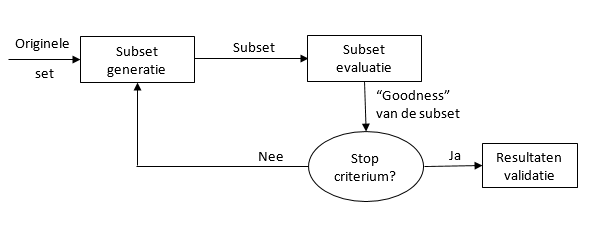
\includegraphics[width=\textwidth]{fig/feature-selection}
\end{figure}

Subset generatie is een zoekprocedure die kandidaat feature subsets produceert voor evaluatie met een bepaalde zoekstrategie. Elke kandidaat subset wordt ge\"evalueerd en vergeleken met de vorige beste volgens een bepaald criterium. Als de nieuwe subset beter is, wordt de vorige beste subset vervangen. Dit proces wordt herhaald tot een bepaald stopcriterium is bereikt. Enkele veel gebruikte stopcriteria zijn: 
\begin{itemize}
\item De zoekopdracht is voltooid
\item Een bepaalde waarde wordt bereikt (minimum aantal features of maximum aantal iteraties)
\item Opeenvolgende toevoeging en verwijdering van features levert geen betere subset op
\item Een voldoende goede subset is gegenereerd (bv. wanneer deze subset in staat is om een classificatieprobleem op te lossen met een bepaalde precisie)
\end{itemize}Dan wordt de geselecteerde beste subset gevalideerd met voorkennis of via verschillende tests op andere datasets. 

\section{Classificatie}
Een eerste techniek die toegepast wordt om een aanbevelingssysteem een beter beeld te geven van de documentencollectie, is classificatie. Door een artikel automatisch aan een categorie te kunnen toewijzen, krijgen we al een veel duidelijker beeld van waarover dit artikel nu precies handelt. Als we zowel de hoofd- als subcategorie van een artikel kunnen bepalen, hebben we al een eerste sterke indicatie of het artikel al dan niet interessant kan zijn voor de gebruiker en dus aanbevolen zal worden door het aanbevelingssysteem. 

\subsection{WEKA}
Om zoveel mogelijk classificatiemethodes te kunnen testen wordt gebruik gemaakt van WEKA \cite{Hall2009} (Waikato Environment for Knowledge Analysis). WEKA is een tool voor datamining ontwikkeld in de programmeertaal Java. Het bestaat uit een grafische werkomgeving  voor het uitvoeren van de nodige stappen bij datamining, een CLI en is volledig ondersteund voor gebruik binnen een eigen Java-programma. Dit framework bevat in totaal 57 verschillende algoritmes om classificatie door te voeren. Deze zijn ingedeeld in verschillende categorie\"en: Bayes, functions, lazy, meta, mi, misc, rules en trees.

De versie van WEKA die gebruikt wordt in deze masterproef is 3.6.13.

De verschillende classifiers binnen WEKA ondersteunen geen meerdere niveaus van classificatie. Om toch gebruik te kunnen maken van een boomstructuur worden de artikels eerst ingedeeld in hun respectievelijke hoofdcategorie\"en en pas daarna in de subcategorie\"en. Omdat het mogelijk is dat voor deze gevallen een andere classifier een beter resultaat oplevert, gaan we deze apart testen. De preprocessing blijft voor alle gevallen gelijk. Wel gaan we eerst uitzoeken welke parameters van de preprocessing het beste beeld geven voor twee Bayesiaanse classifiers. 

In eerste instantie wordt gefocust op de dataset van Het Laatste Nieuws. Vervolgens wordt met de gevonden inzichten en nieuwe classificatie toegepast op een tweede dataset van Wikipedia. 

\subsection{Preprocessing in WEKA}
In WEKA wordt voor preprocessing van de documentencollectie de functie \textit{string-to-wordvector} gebruikt. Deze functie converteert de teksten naar een set van attributen die het aandeel van dat attribuut voorstellen in de documentencollectie. 

De string-to-word functie in WEKA neemt een aantal parameters. Een eerste parameter is de tokenizer functie. Deze bepaalt hoe een tekst wordt opgesplitst in woorden. Hier wordt gebruik gemaakt van een N-Gram tokenizer. Deze geeft de mogelijkheid om eventueel twee of drie woorden samen te nemen en als \'e\'en woord in de documentencollectie te zien.

Ten tweede kan gekozen worden voor term frequency-inverse document frequency (tf-idf), al dan niet gecombineerd met een normalisatie. De achterliggende logica zit vervat in formule \ref{eq:tfidf}. Op deze manier worden termen die belangrijk zijn voor een document, maar minder vaak of niet in de volledige documentencollectie voorkomen, een groter gewicht toegekend in de vector representatie. 

Een derde parameter die ingesteld kan worden is het gebruikte stemmingsalgoritme.  Op basis van de metadata gegenereerd door Apache Tika (sectie \ref{tika}) kan hier dynamisch een alternatieve stemmer gekozen worden per taal. Hier werd een Nederlandstalige stemmer gebruikt, zoals beschreven in \cite{Kraaij1994} (aangezien Nederlandse datasets gebruikt worden). Deze stemmer is een uitbreiding van het originele stemmingsalgoritme van Porter, zoals voorgesteld in \cite{Porter1980}, naar de Nederlandse taal. 

Een vierde parameter is de stopwoordfilter. Hiervoor wordt een lijst met stopwoorden gebruikt voor de Nederlandse taal. De stopwoordfilter zorgt ervoor dat woorden die veel voorkomen in een taal, maar relatief weinig inhoud hebben, niet overwogen worden om op te nemen in het woordenboek. Denk daarbij aan 'de', 'het', 'daar', 'dan', etc. Na de fase van tokenization kunnen deze woorden weggefilterd worden, zodat ze geen negatieve invloed hebben op het uiteindelijk resultaat.

Een vijfde parameter laat toe om de frequentie van een woord uit te drukken, in plaats van binaire aanwezigheid. Hierdoor wordt de belangrijkheid van bepaalde woorden soms meer in de verf gezet.

De laatste parameter is het aantal woorden dat behouden wordt per klasse uit de documentencollectie. Dit is natuurlijk een belangrijke parameter, omdat meer betekenisvolle woorden in het woordenboek naar een betere classificatie en/of clustering zullen leiden. Als we echter te veel woorden opnemen, waardoor er een bepaalde ruis gaat optreden, krijgen we ook slechts een suboptimale werking. Het is echter moeilijk om zomaar te bepalen hoeveel woorden een optimale classificatie zullen geven bij elke methode. Bovendien is het mogelijk dat het voor onze dataset niet nuttig is om een stemmer of stopwoordfilter te gaan gebruiken. Daarom wordt in sectie \ref{parameters-voor-preprocessing} een benchmark opgesteld die het optimale aantal woorden gaat onderzoeken bij classificatie. Verder wordt daar ook het nut van de stemmer en van de stopwoordfilter verder onderzocht. Ook wordt het effect van deze parameters op de uiteindelijke classificatie geanalyseerd. 
In sectie \ref{IG} komen we terug op feature selection. Er wordt onderzocht of deze functie inderdaad een positief effect kan hebben op de effectieve classificatie.

\subsection{Parameters voor preprocessing van data}\label{parameters-voor-preprocessing}

Om de optimale parameters voor de preprocessing te bepalen wordt een classificatie uitgevoerd met de verwerkte dataset. We vari\"eren de parameters en bepalen zo de optimale instellingen. De dataset die eerst gebruikt wordt is deze van Het Laatste Nieuws, januari 2008. De classifiers die gebruikt worden om de bekomen woordvector te testen zijn \quotes{Naive Bayes} en \quotes{Naive Bayes Multinomial}. 

Om een betrouwbaar resultaat te bekomen worden de tests met een \textit{10-fold cross validation}\label{10-fold-cv} \cite{Bengio2004} uitgevoerd. Dit is een techniek om voorspellende modellen te evalueren door de originele dataset te verdelen in een trainingsset om het model te trainen en een testset om deze te valideren. Bij 10-fold cross-validation\label{cross-val} wordt de originele dataset random verdeeld in 10 subsets. Daarvan wordt \'e\'en subset behouden ter validatie van het model. De overige 9 subsets worden gebruikt als trainingsdata. Het cross-validation proces wordt 10 keer herhaald, waarbij elk van de subsets exact \'e\'en keer gebruikt worden als validatieset. De 10 resultaten worden gecombineerd (uitgemiddeld) om een enkele voorspelling te maken. Het grote voordeel van deze methode is dat alle observaties zowel als trainings- en als validatiedata kunnen worden gebruikt. 

Om de resultaten onafhankelijk te stellen van het aantal woorden die behouden worden van de documentencollectie, wordt gebruikt gemaakt van de standaard bijgehouden 1000 woorden. Deze parameter wordt in de volgende secties per dataset apart geverifieerd. We gaan er immers van uit dat er voor de classificatie op het eerste niveau van de boom meer woorden zullen nodig zijn om alle items correct te kunnen classificeren dan op het tweede niveau. Het lagere niveau bevat immers al tekst die specifiek is voor die categorie en heeft dus een minder uitgebreide woordenschat. Verder worden de verschillende parameters al dan niet ingesteld, zoals te zien in tabel \ref{tab:preprocessing-params}. Hierbij staat \quotes{1} voor \quotes{gebruikt} en \quotes{0} voor \quotes{niet gebruikt}.

\LTcapwidth=\textwidth
\begin{longtable}{rrrrrrr}
	\caption{Gebruik van verschillende parameters bij preprocessing van de documentencollectie \quotes{Het Laatste Nieuws, januari 2008} en hun effect op het percentage correct geclassificeerde artikels volgens de \quotes{Naive Bayes} (NB) en \quotes{Naive Bayes Multinomial} (NBM) classifiers in hoofdcategorie\"en.}\\
	\toprule
	\multicolumn{1}{c}{\textbf{tf-idf}} & \multicolumn{1}{c}{\textbf{Stemming}} & \multicolumn{1}{c}{\textbf{Stopwoorden}} & \multicolumn{1}{c}{\textbf{Frequentie}} & \multicolumn{1}{c}{\textbf{Tokenizer}} & \multicolumn{1}{c}{\textbf{NB}} & \multicolumn{1}{c}{\textbf{NBM}} \\
	\midrule
	0     & 0     & 0     & 0     & 1     & 69.85\% & 74.39\% \\
	0     & 0     & 0     & 0     & 2     & 67.62\% & 72.34\% \\
	0     & 0     & 0     & 0     & 3     & 67.44\% & 72.15\% \\
	0     & 0     & 0     & 1     & 1     & 56.06\% & 66.39\% \\
	0     & 0     & 0     & 1     & 2     & 54.26\% & 64.35\% \\
	0     & 0     & 0     & 1     & 3     & 54.24\% & 64.30\% \\
	0     & 0     & 1     & 0     & 1     & 71.50\% & 75.71\% \\
	0     & 0     & 1     & 0     & 2     & 69.26\% & 73.41\% \\
	0     & 0     & 1     & 0     & 3     & 68.91\% & 73.09\% \\
	0     & 0     & 1     & 1     & 1     & 58.01\% & 68.31\% \\
	0     & 0     & 1     & 1     & 2     & 56.25\% & 66.18\% \\
	0     & 0     & 1     & 1     & 3     & 56.20\% & 66.09\% \\
	0     & 1     & 0     & 0     & 1     & 70.85\% & 75.43\% \\
	0     & 1     & 0     & 0     & 2     & 68.19\% & 72.65\% \\
	0     & 1     & 0     & 0     & 3     & 68.35\% & 72.61\% \\
	0     & 1     & 0     & 1     & 1     & 57.68\% & 67.55\% \\
	0     & 1     & 0     & 1     & 2     & 55.74\% & 65.36\% \\
	0     & 1     & 0     & 1     & 3     & 55.88\% & 65.43\% \\
	0     & 1     & 1     & 0     & 1     & \textbf{71.91\%} & \textbf{76.37\%} \\
	0     & 1     & 1     & 0     & 2     & 69.44\% & 73.82\% \\
	0     & 1     & 1     & 0     & 3     & 69.42\% & 73.70\% \\
	0     & 1     & 1     & 1     & 1     & 59.09\% & 69.31\% \\
	0     & 1     & 1     & 1     & 2     & 57.49\% & 67.30\% \\
	0     & 1     & 1     & 1     & 3     & 57.29\% & 67.07\% \\
	1     & 0     & 0     & 0     & 1     & 36.40\% & 57.44\% \\
	1     & 0     & 0     & 0     & 2     & 40.78\% & 58.42\% \\
	1     & 0     & 0     & 0     & 3     & 40.85\% & 58.31\% \\
	1     & 0     & 0     & 1     & 1     & 40.88\% & 59.59\% \\
	1     & 0     & 0     & 1     & 2     & 45.99\% & 60.97\% \\
	1     & 0     & 0     & 1     & 3     & 45.68\% & 60.59\% \\
	1     & 0     & 1     & 0     & 1     & 34.45\% & 56.63\% \\
	1     & 0     & 1     & 0     & 2     & 39.73\% & 58.00\% \\
	1     & 0     & 1     & 0     & 3     & 39.73\% & 57.79\% \\
	1     & 0     & 1     & 1     & 1     & 38.56\% & 58.81\% \\
	1     & 0     & 1     & 1     & 2     & 43.64\% & 59.91\% \\
	1     & 0     & 1     & 1     & 3     & 43.97\% & 59.96\% \\
	1     & 1     & 0     & 0     & 1     & 38.92\% & 59.00\% \\
	1     & 1     & 0     & 0     & 2     & 42.52\% & 59.58\% \\
	1     & 1     & 0     & 0     & 3     & 42.72\% & 59.59\% \\
	1     & 1     & 0     & 1     & 1     & 43.99\% & 61.61\% \\
	1     & 1     & 0     & 1     & 2     & 47.16\% & 62.01\% \\
	1     & 1     & 0     & 1     & 3     & 47.29\% & 61.88\% \\
	1     & 1     & 1     & 0     & 1     & 37.17\% & 58.58\% \\
	1     & 1     & 1     & 0     & 2     & 41.38\% & 59.36\% \\
	1     & 1     & 1     & 0     & 3     & 41.70\% & 59.37\% \\
	1     & 1     & 1     & 1     & 1     & 41.78\% & 60.86\% \\
	1     & 1     & 1     & 1     & 2     & 45.68\% & 61.52\% \\
	1     & 1     & 1     & 1     & 3     & 46.10\% & 61.64\% \\
	\bottomrule
	\label{tab:preprocessing-params}
\end{longtable}%

De tabel leert ons dat een combinatie van een N-Gram tokenizer van maximum 1 woord, het stemmingsalgoritme en de stopwoordfiltering leidt tot het beste resultaat voor beide classificaties. Als we de frequentie weergeven in de woordvector, dan leidt dit meestal tot een daling van het aantal correct geclassificeerde documenten, terwijl de term frequency-inverse document frequency het aantal correct geclassificeerde documenten nog sterker doet dalen. Dit is een opmerkelijke vaststelling die niet lijkt te stroken met de verwachtingen. Mogelijke verklaringen voor dit fenomeen zijn dat de belangrijke termen in teksten van Het Laatste Nieuws niet veelvuldig gebruikt worden in artikels. Dit is bijvoorbeeld zo voor artikels waar de eerste minister vermeld wordt. De naam van de eerste minister wordt slechts \'e\'en maal vermeld in het artikel en vervolgens telkens vervangen door synoniemen en verwijzingen zoals \quotes{de eerste minister}, \quotes{de premier}, \quotes{Charles Michel}, etc. Het zou daarom kunnen dat andere woorden vaker voorkomen dan de eigenlijk typerende woorden voor dit artikel, waardoor een term frequency-inverse document frequency eigenlijk de belangrijkheid van deze termen onderdrukt. Een mogelijke oplossing voor dit probleem zou \textit{synonym detection} (bv. \cite{Zesch2008}, \cite{Weale2009}) zijn. Verschillende andere oplossingen gaan met behulp van bestaande woordenboeken of encyclopedie\"en (bv. \cite{Cheng2013}) op zoek naar termen die gelijkaardig zijn. Deze technieken vallen echter buiten de scope van dit onderzoek en zijn bovendien nog weinig onderzocht voor Nederlandstalige teksten. 

Om het vector space model op te stellen voor de dataset van Het Laatste Nieuws, gaan we dus een N-Gram tokenizer van 1 woord gebruiken en zowel stemming als stopwoordfiltering toepassen. Term frequency-inverse document frequency en frequentie van woorden gebruiken we niet.

Ook voor de dataset van Wikipedia worden de optimale parameters voor preprocessing bepaald op dezelfde manier. De resultaten zijn te vinden in tabel \ref{tab:preprocessing-wiki}

\LTcapwidth=\textwidth
\begin{longtable}{rrrrrrr}
	\caption{Gebruik van verschillende parameters bij preprocessing van de documentencollectie \quotes{Wikipedia} en hun effect op het percentage correct geclassificeerde artikels volgens de \quotes{Naive Bayes} (NB) en \quotes{Naive Bayes Multinomial} (NBM) classifiers in hoofdcategorie\"en.}\\
	\toprule
	\multicolumn{1}{c}{\textbf{tf-idf}} & \multicolumn{1}{c}{\textbf{Stemming}} & \multicolumn{1}{c}{\textbf{Stopwoorden}} & \multicolumn{1}{c}{\textbf{Frequentie}} & \multicolumn{1}{c}{\textbf{Tokenizer}} & \multicolumn{1}{c}{\textbf{NB}} & \multicolumn{1}{c}{\textbf{NBM}} \\
	\midrule
0	& 0	& 0	& 0	& 1	& 34.80\%	& 37.56\% \\
0	& 0	& 0	& 0	& 2	& 33.08\%	& 35.53\% \\
0	& 0	& 0	& 0	& 3	& 32.56\%	& 35.04\% \\
0	& 0	& 0	& 1	& 1	& 28.24\%	& 33.54\% \\
0	& 0	& 0	& 1	& 2	& 28.46\%	& 32.89\% \\
0	& 0	& 0	& 1	& 3	& 28.26\%	& 32.63\% \\
0	& 0	& 1	& 0	& 1	& 36.09\%	& 39.40\% \\
0	& 0	& 1	& 0	& 2	& 33.86\%	& 36.71\% \\
0	& 0	& 1	& 0	& 3	& 33.69\%	& 36.23\% \\
0	& 0	& 1	& 1	& 1	& 30.36\%	& 35.24\% \\
0	& 0	& 1	& 1	& 2	& 29.16\%	& 33.62\% \\
0	& 0	& 1	& 1	& 3	& 28.42\%	& 33.17\% \\
0	& 1	& 0	& 0	& 1	& 35.53\%	& 38.35\% \\
0	& 1	& 0	& 0	& 2	& 33.79\%	& 36.41\% \\
0	& 1	& 0	& 0	& 3	& 33.41\%	& 35.83\% \\
0	& 1	& 0	& 1	& 1	& 27.97\%	& 34.04\% \\
0	& 1	& 0	& 1	& 2	& 28.56\%	& 33.42\% \\
0	& 1	& 0	& 1	& 3	& 28.46\%	& 33.30\% \\
0	& 1	& 1	& 0	& 1	& 36.23\%	& 39.65\% \\
0	& 1	& 1	& 0	& 2	& 34.61\%	& 37.81\% \\
0	& 1	& 1	& 0	& 3	& 34.08\%	& 37.12\% \\
0	& 1	& 1	& 1	& 1	& 29.86\%	& 35.49\% \\
0	& 1	& 1	& 1	& 2	& 29.59\%	& 34.69\% \\
0	& 1	& 1	& 1	& 3	& 29.19\%	& 34.49\% \\
1	& 0	& 0	& 0	& 1	& 37.03\%	& 40.22\% \\
1	& 0	& 0	& 0	& 2	& 35.29\%	& 38.33\% \\
1	& 0	& 0	& 0	& 3	& 34.36\%	& 37.67\% \\
1	& 0	& 0	& 1	& 1	& 37.97\%	& 41.06\% \\
1	& 0	& 0	& 1	& 2	& 37.00\%	& 39.78\% \\
1	& 0	& 0	& 1	& 3	& 35.53\%	& 38.86\% \\
1	& 0	& 1	& 0	& 1	& 37.38\%	& 40.54\% \\
1	& 0	& 1	& 0	& 2	& 35.57\%	& 38.57\% \\
1	& 0	& 1	& 0	& 3	& 34.52\%	& 37.84\% \\
1	& 0	& 1	& 1	& 1	& 38.32\%	& 41.46\% \\
1	& 0	& 1	& 1	& 2	& 36.69\%	& 39.77\% \\
1	& 0	& 1	& 1	& 3	& 35.99\%	& 39.18\% \\
1	& 1	& 0	& 0	& 1	& 37.89\%	& 40.91\% \\
1	& 1	& 0	& 0	& 2	& 36.11\%	& 39.53\% \\
1	& 1	& 0	& 0	& 3	& 35.14\%	& 38.70\% \\
1	& 1	& 0	& 1	& 1	& 38.82\%	& 41.82\% \\
1	& 1	& 0	& 1	& 2	& 37.47\%	& 40.65\% \\
1	& 1	& 0	& 1	& 3	& 36.11\%	& 39.74\% \\
1	& 1	& 1	& 0	& 1	& 37.87\%	& 40.99\% \\
1	& 1	& 1	& 0	& 2	& 36.51\%	& 39.95\% \\
1	& 1	& 1	& 0	& 3	& 35.24\%	& 38.89\% \\
1	& 1	& 1	& 1	& 1	& \textbf{39.27}\%	& \textbf{42.28}\% \\
1	& 1	& 1 & 1	& 2	& 37.64\%	& 40.94\% \\
1	& 1	& 1	& 1	& 3	& 36.26\%	& 40.01\% \\
	\bottomrule
	\label{tab:preprocessing-wiki}
\end{longtable}%

Er kan opgemerkt worden dat over hele lijn, onafhankelijk van de ingestelde parameters, het aantal correct geclassificeerde artikels een stuk lager ligt dan bij Het Laatste Nieuws het geval was. Een mogelijke verklaring ligt in het feit dat de dataset van Wikipedia zo is opgebouwd dat deze per categorie evenveel artikels bevat. Als een classifier dus niet zeker is waar een bepaald artikel terecht moet komen en bijgevolg gaat gokken, heeft het systeem maar een kans van 1 op 9 om het artikel alsnog in een juiste categorie onder te brengen. Als we dit vergelijken met Het Laatste Nieuws zien we daar 11 categorie\"en. De verdelingen van de artikels over die categorie\"en is echter niet evenredig. Als een classifier bij deze dataset niet zeker is waar een artikel thuishoort, dan gokt hij op de categorie waar de meeste artikels inzitten. Voor de datset van januari 2008 bevat de categorie nieuws 31,69\% van alle artikels, wat dus een kans van bijna 1 op 3 vertegenwoordigd. Het is dus logisch dat een classifier bij de dataset van Wikipedia een beduidend lagere score haalt voor het aantal correct geclassificeerde artikels.

Een andere verklaring voor dit fenomeen is dat de categorie\"en waarin de artikels van Wikipedia werden ingedeeld veel minder afgebakend zijn dan bij Het Laatste Nieuws. In principe is de structuur van Wikipedia opgebouwd als een hi\"erarchie, weergegeven volgens een acyclische verbonden graaf \cite{Milne2007}. Deze structuur lijkt op een boomstructuur, maar iedere knoop kan verbonden zijn met verschillende andere knopen rondom zich. Er zitten bijgevolg veel overlappingen tussen de categorie\"en en er komen zelfs circulaire referenties terug. Als we bijvoorbeeld een categorie \quotes{cultuur} beschouwen vinden we daar artikels over o.a. voeding. Mochten we de graaf voor categorie voeding opstellen krijgen we ongeveer de figuur in \ref{fig:wiki-voeding}\footnote{\url{https://tools.wmflabs.org/vcat/catgraphRedirect?wiki=nlwiki&cat=Voeding&format=png&links=wiki}}.

\begin{figure}[h]
	\caption{Hi\"erarchie binnen Wikipedia van de categorie voeding\protect}
	\label{fig:wiki-voeding}	
	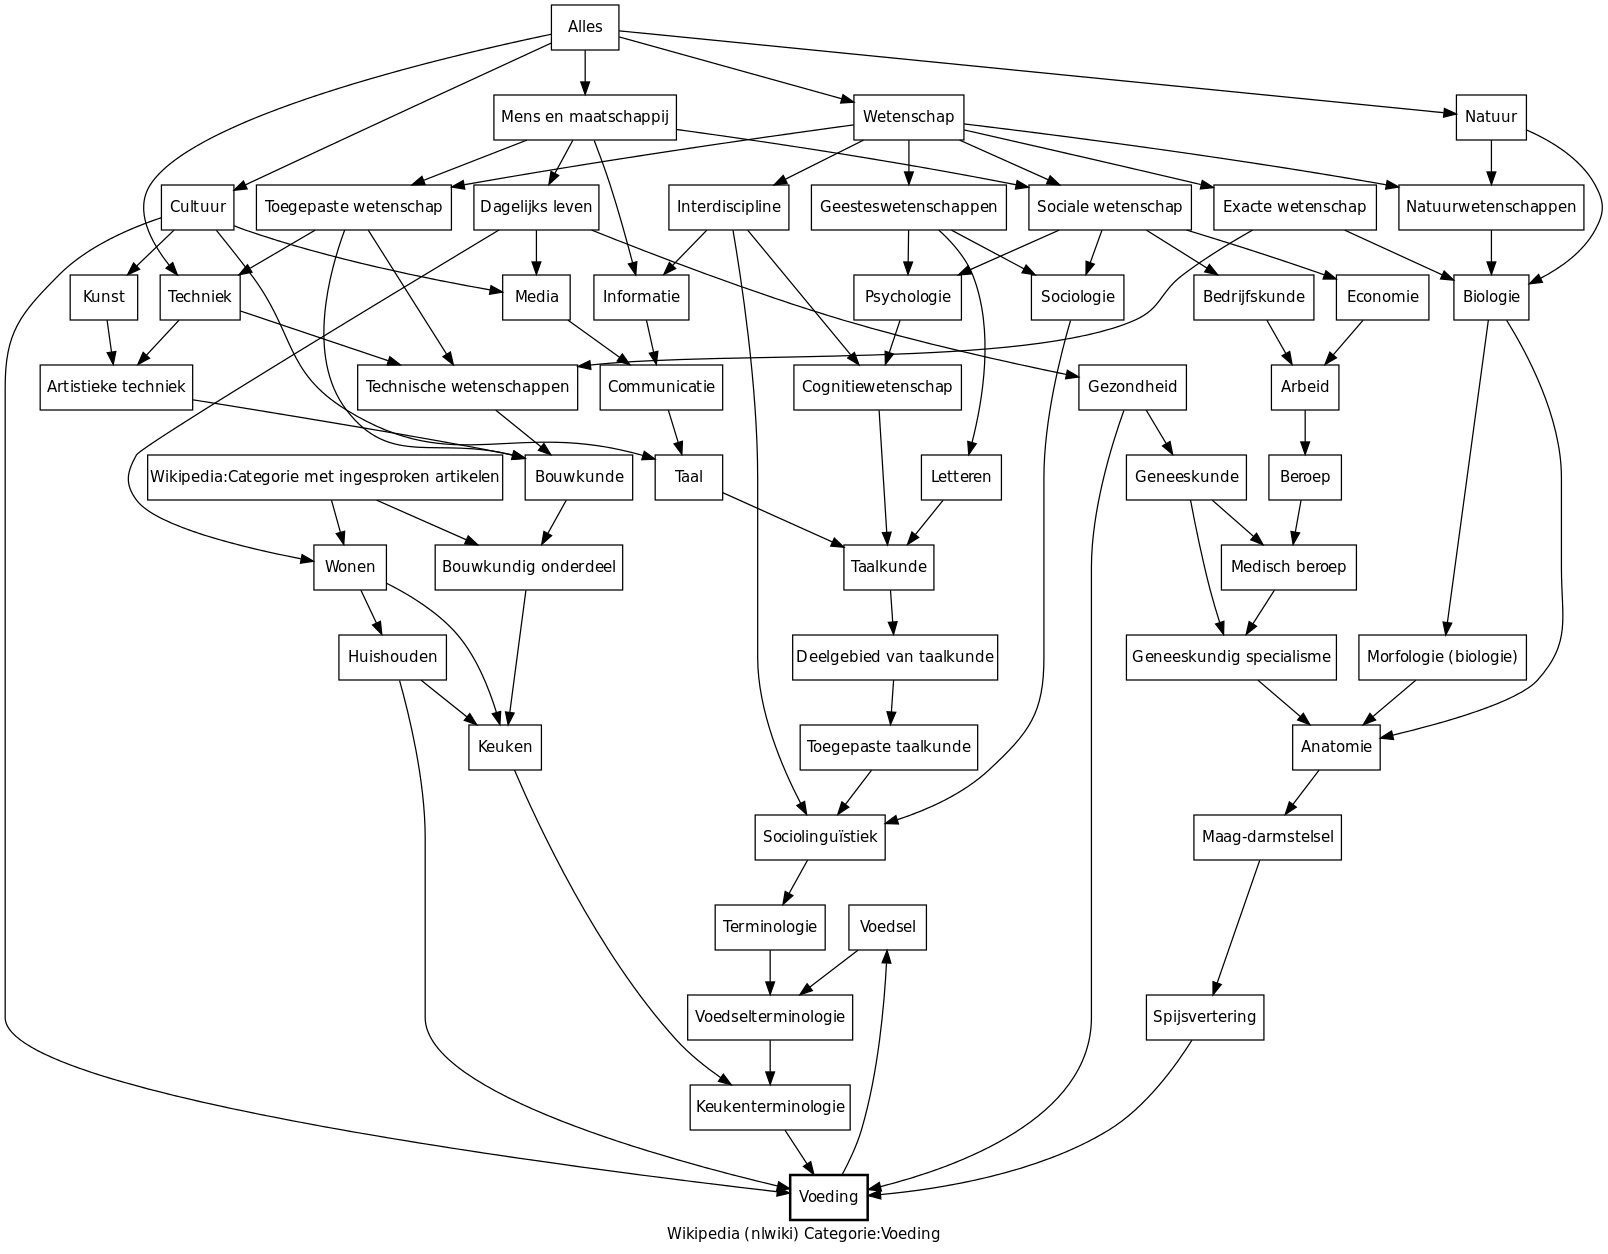
\includegraphics[width=\textwidth]{fig/voeding.png}
\end{figure}

Deze figuur toont hoe de categorie voeding niet enkel onder hoofdcategorie cultuur staat, maar ook onder hoofdcategorie\"en \quotes{mens en maatschappij}, \quotes{wetenschap}, \quotes{natuur}, etc. Het is bijgevolg al een goed resultaat dat bepaalde artikels in wezen ingedeeld worden in een correcte structuur. De resultaten van deze dataset vallen dan ook moeilijk te vergelijken met deze van Het Laatste Nieuws, waar wel een duidelijke boomstructuur van 2 niveaus wordt gebruikt. De verdere resultaten van classificatie van deze artikels kunnen gevonden worden in sectie \ref{clas:wiki}.

Als vervolgens gefocust wordt op de preprocessing parameters, valt op dat hier term frequency-inverse document frequency wel een positief resultaat oplevert. De optimale preprocessing parameters voor deze dataset liggen meer in de lijn van verwachting dan deze van het laatste nieuws, aangezien alle mogelijkheden van de preprocessing bijdragen tot een beter resultaat van classificatie. Er wordt bijgevolgd bij preprocessing van deze dataset zowel tf-idf, stemming, stopwoordfiltering, woordfrequentie en tokenization met 1 NGram gebruikt om tot een optimale classificatie te kunnen komen.

\subsection{Feature selection}\label{IG}
Feature selection probeert om een subset van de features te zoeken die relevant zijn voor het doelconcept. Het wordt op verschillende manieren beschreven, maar voor deze use case zijn de criteria de volgende:
\begin{itemize}
\item De nauwkeurigheid van de classificatie daalt niet of nauwelijks,
\item De resulterende klassenverdeling ligt zo dicht mogelijk bij de originele klassenverdeling, gegeven alle features.
\end{itemize}

Om aan deze voorwaarden te voldoen gebruiken we het Information Gain (IG) algoritme \cite{Liu2005}. Dit algoritme werkt als volgt: stel dat $P_i$ de globale probabiliteit is van klasse $i$ voorstelt, en $p_{i}(w)$ de probabiliteit van klasse $i$ als het document het woord $w$ bevat. $F(w)$ is dan de fractie van de documenten die het woord $w$ bevatten. Information Gain $I(w)$ is als volgt gedefinieerd voor een gegeven woord  $w$:

\begin{equation}
I(w) = -\sum_{i=1}^{k}P_i\cdot\log{(P_i)} + F(w)\cdot\log(p_i(w)) + (1 - F(w))\cdot\sum_{i=1}^{k}(1-p_i(w))\cdot\log(1-p_i(w))
\end{equation}

Hoe groter de waardes voor IG $I(w)$, hoe groter de discriminerende kracht van het woord $w$ \cite{Forman2003}.

We testen de implementatie van IG uit  in combinatie met het Ranker-algoritme in WEKA, op het woordenboek met de gekozen opties bij preprocessing voor de dataset van Het Laatste Nieuws. Dit levert de resultaten in tabel \ref{tab:feature-selection}.

\begin{table}[htbp]
	\centering
	\caption{Vergelijking voor en na feature selection met de Information Gain-methode voor dataset Het Laatste Nieuws, januari 2008}
	\begin{tabular}{rrrrrrr}
		\toprule
		\multicolumn{3}{c}{\textbf{Origineel}} & \multicolumn{1}{c|}{\textbf{}} & \multicolumn{3}{c}{\textbf{Information Gain}} \\
		\midrule
		\textbf{NB} & \textbf{NBM} & \textbf{woorden}    &   \multicolumn{1}{c|}{}   & \textbf{NB} & \textbf{NBM} & \textbf{woorden} \\
		71.91\% & 76.37\% & 1000  &   \multicolumn{1}{c|}{}    & 72.01\% & 76.51\% & 893 \\
		\bottomrule
	\end{tabular}%
	\label{tab:feature-selection}%
\end{table}%

We merken een sterke daling in het aantal woorden (10,70\%), maar tergelijkertijd een lichte stijging in het aantal juist geclassificeerde documenten (voor de "Naive Bayes$"$ classifier 0,10\%, voor de "Naive Bayes Multinomial" classifier 0,14\%).  We kunnen hier dus besluiten dat IG een algoritme is dat goede resultaten geeft voor deze tekstuele data. De zogenaamde ruis wordt weggenomen uit de woordvector en de belangrijkste woorden werden behouden.

Als we diezelfde IG toepassen op de dataset van Wikipedia krijgen we de resultaten in tabel \ref{tab:feature-selection-wiki}.

\begin{table}[htbp]
	\centering
	\caption{Vergelijking voor en na feature selection met de Information Gain-methode voor dataset Wikipedia}
	\begin{tabular}{rrrrrrr}
		\toprule
		\multicolumn{3}{c}{\textbf{Origineel}} & \multicolumn{1}{c|}{\textbf{}} & \multicolumn{3}{c}{\textbf{Information Gain}} \\
		\midrule
		\textbf{NB} & \textbf{NBM} & \textbf{woorden}    &   \multicolumn{1}{c|}{}   & \textbf{NB} & \textbf{NBM} & \textbf{woorden} \\
		39.26\% & 42.27\% & 1000  &   \multicolumn{1}{c|}{}    & 34.93\% & 44.92\% & 600 \\
		\bottomrule
	\end{tabular}%
	\label{tab:feature-selection-wiki}%
\end{table}%

Bij deze dataset merken we een heel sterke daling in het aantal woorden op (40 \%). Dit duidt op het feit dat veel woorden gevonden worden die weinig bijdragen tot een categorie. Ook dit kan herleid worden naar het feit dat de classifier er moeite mee heeft een eenduidige definitie op te stellen van een categorie. Ondanks de sterke daling in woorden zien we een stijging in het aantal correct geclassificeerde artikels voor de NBM-methode (2,65\%). Voor de na\"ieve Bayesiaanse methode merken we wel een daling op van 4,33 \%. Ondanks deze daling bewijst het IG algoritme zijn nut door het aantal woorden sterk te doen dalen en tegelijkertijd een stijging in het aantal correct geclassificeerde artikels te bekomen voor de NBM-methode.

\subsection{Classificatie in hoofdcategorie\"en (dataset Het Laatste Nieuws)}
Er wordt gestart met het classificeren in hoofdcategorie\"en. De dataset van januari 2008 bevat 11 hoofdcategorie\"en: Auto, Bizar, Geld, iHLN, Muziek, Nieuws, Reizen, Showbizz, Sport, Wetenschap en You. De verdeling van de artikels over deze hoofdcategorie\"en kan gevonden worden in tabel \ref{tab:hln-2008-01-cat}.

Om de best mogelijke classificatie te vinden, wordt een testbank opgesteld waarin een selectie van algoritmes voor classificatie in WEKA (46) opgenomen zijn. Enkele classifiers werden niet opgenomen omdat ze o.a. manuele input verwachten. Omdat dit een geautomatiseerde toepassing is kunnen deze algoritmes niet manueel verwerkt worden. De gekozen classifiers worden met de standaardopties uitgevoerd op de data van Het Laatste nieuws uit januari 2008, die vooraf door de preprocessing-fase gegaan is. De classifiers worden vervolgens gerangschikt volgens het percentage correct geclassificeerde artikels, gebruik makend van een 10-fold cross-validation (zie \ref{10-fold-cv}).

\subsubsection{Na\"ieve baseline classifier}\label{naieve-classifier}
Het aantal woorden die opgenomen wordt in de preprocessing van de documentencollectie wordt gevarieerd van 100 t.e.m. 20000 attributen met telkens een increment van 100 attributen. Nadien wordt de Information Gain methode (zie \ref{IG}) toegepast om eventuele ruis te verwijderen. Al snel - na 2000 attributen - merken we echter dat enkele methodes het heel erg slecht doen. Een eerste zeer na\"ieve classifier waarmee vergeleken wordt is een classifier die alle artikels toekent aan de categorie met het meeste artikels (in dit geval nieuws). Deze na\"ieve implementatie zal in principe 31,69\% correct classificeren. In WEKA wordt deze ge\"implementeerd onder de naam ZeroR. Dit algoritme is ook opgenomen in lijst van classifiers. 

\iffalse
\begin{table}[htbp]
	\centering
	\caption{Classifiers die het slechter of even goed doen als de na\"ieve baseline classifier (ZeroR) bij classificatie van artikels in hoofdcategorie\"en na bijhouden van 2000 woorden in de woordvector.}
	\begin{tabular}{rrr}
		\toprule
		& 1000  & 2000 \\
		\midrule
		CVParameterSelection & \multicolumn{1}{c}{31.70\%} & \multicolumn{1}{c}{31.70\%} \\
		Grading & \multicolumn{1}{c}{31.70\%} & \multicolumn{1}{c}{31.70\%} \\
		MultiScheme & \multicolumn{1}{c}{31.70\%} & \multicolumn{1}{c}{31.70\%} \\
		Stacking & \multicolumn{1}{c}{31.70\%} & \multicolumn{1}{c}{31.70\%} \\
		StackingC & \multicolumn{1}{c}{31.70\%} & \multicolumn{1}{c}{31.70\%} \\
		Vote  & \multicolumn{1}{c}{31.70\%} & \multicolumn{1}{c}{31.70\%} \\
		ZeroR & \multicolumn{1}{c}{31.70\%} & \multicolumn{1}{c}{31.70\%} \\
		VFI   & \multicolumn{1}{c}{13.02\%} & \multicolumn{1}{c}{8.93\%} \\
		\bottomrule
	\end{tabular}%
	\label{tab:naive-classifiers}%
\end{table}
\fi

Als we ZeroR als baseline classifier beschouwen om te bepalen wat een slechte classifier is, dan vinden we enkele methodes die deze baseline niet halen en die het m.a.w. slechter of net even goed doen als ZeroR bij 2000 woorden. De zwakke classifiers zijn VFI (Voting Feature Intervals), Vote, Stacking, StackingC, MultiScheme, Grading, CVParameterSelection en ClassificationViaClustering. Als we enkele van deze algoritmes van dichterbij gaan bekijken, zien we dat o.a. Vote, VFI, Stacking, StackingC, MultiScheme en Grading enkele extra parameters verwachten waarin (enkele) andere classifiers worden opgegeven. Die methodes gaan dus andere classifiers combineren en enkelen hiervan worden verder besproken in \ref{combineren-classifiers}, waar de voordelen van het combineren van classifiers wordt onderzocht. 

Het is voor verder onderzoek naar de beste classifiers voor deze dataset niet nuttig dat de vermelde classifiers verder individueel onderzocht worden. Om rekenkracht te sparen worden deze dan ook niet meer opgenomen in de resultaten na 2000 woorden.

\subsubsection{Top 10 classifiers}
Na 2000 woorden wordt bovendien een top 10 van beste classifiers opgesteld. Criteria  voor selectie zijn methodes die steeds verbeteren als het aantal woorden wordt opgedreven en methodes die binnen maximum 2 uur een oplossing kunnen vinden. Op die manier kan sneller en gemakkelijker vergeleken worden. Grafiek \ref{fig:clas-20000} toont de vijf beste  classifiers en het punt waar hun optimale classificatie bereikt wordt. Het is duidelijk dat de classifier DMNBText hier het best presteert vanaf 15500 woorden (89,86\% correct geclassificeerd). De classifier Logistic heeft vanaf 2000 woorden geen geheugen meer genoeg om verdere classificatie toe te staan, maar presteert wel voldoende goed bij weinig woorden om in de top 10 te worden opgenomen.

\begin{figure}[h]
	\caption{Top 5 classifiers voor classificatie van dataset Het Laatste Nieuws in hoofdcategorie\"en}
	\label{fig:clas-20000}	
	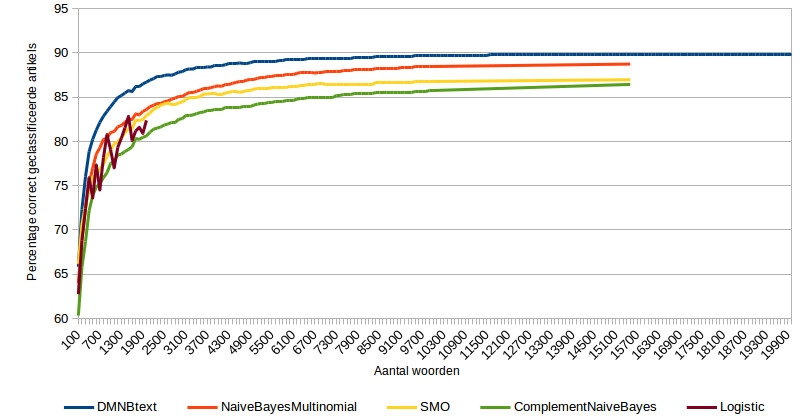
\includegraphics[width=\textwidth]{fig/classificatie-20000-hln.jpeg}
\end{figure}

\subsection{Combineren van classifiers voor hoofdcategorie\"en}
\label{combineren-classifiers}
Het is mogelijk dat we door verschillende goede individuele classifiers te combineren, een betere algemene classificatie bekomen. Om die stelling te onderzoeken worden drie combinatiealgoritmes getest in de volgende paragrafen: voting, stacking en grading.

\subsubsection{Voting}
Het algoritme dat eerst gebruikt wordt is \quotes{Vote} \cite{Kittler1998}. Dit is een algoritme dat zelfstandig geen classificatie uitvoert (zie ook resultaten individuele classifiers, \ref{naieve-classifier}). Het neemt een aantal zelf gekozen classifiers samen en laat die stemmen om te bepalen tot welke klasse een bepaald document behoort. Om er zeker van te zijn of dit een effectieve verbetering oplevert passen we het "Vote$"$-algoritme toe met de top 4 beste algoritmes voor classificatie in hoofdcategorie\"en: DMNBText, MultinomialNaiveBayes, SMO en ComplementNaiveBayes. 

\begin{table}[htbp]
	\centering
	\caption{Aantal correct geclassificeerde artikels bij gebruik van het Vote-algoritme met classifiers DMNBText, MultinomialNaiveBayes, SMO en ComplementNaiveBayes voor dataset Het Laatste Nieuws (januari 2008) met verschillende combinatiemethodes.}
	\begin{tabular}{rr}
		\toprule
		Combinatiemethode & Correct geclassificeerd \\
		\midrule
		Average of Probabilities & 89,65\% \\
		Product of Probabilities & 86,45\% \\
		Majority Voting & 89,92\% \\
		Minimum Probability & 86,45\% \\
		Maximum Probability & 86,56\% \\
		\bottomrule
	\end{tabular}%
	\label{tab:vote}%
\end{table}%

Het Vote-algoritme laat toe om met verschillende methodes de originele classificaties te combineren. Deze worden voorgesteld in tabel \ref{tab:vote}, samen met het percentage correct geclassificeerde artikels voor de preprocessed dataset van januari 2008.

De methode \quotes{Majority Voting} geeft een licht beter resultaat dan de beste individuele classifier (DMNBText; 89,86\% correct geclassificeerd). Het verschil is dan wel heel klein (0,06\%), maar toch significant aangezien deze classifier op een dataset van bijvoorbeeld 10000 artikels toch 600 artikels meer correct zou kunnen classificeren. 

\subsubsection{Stacking}\label{stacking}
Een andere methode om mogelijk een beter classificatie te bekomen is het \quotes{Stacking}-algoritme. Meestal presteert dit beter dan voting \cite{Sigletos2005}. Stacking wordt gezien als een generalisatie van het "Vote$"$-algoritme. Het combineert de voorspellingen van verschillende andere classifiers en past een zelfgekozen combinatie-algoritme toe met de voorspellingen van de andere algoritmes als extra input. 

Het combineert meerdere classifiers die gegenereerd zijn door verschillende lerende algoritmes $L_1$,...,$L_n$ op een dataset S toe te passen. De dataset bestaat uit elementen in de vorm van $s_i = (x_i, y_i)$, welke in dit geval de paren van de feature vectoren ($x_i$) met hun classificatie ($y_i$) voorstellen. In de eerste fase worden base-level classifiers $C_1$,...,$C_n$ gegenereerd, waar $C_i = L_{i}(S)$. In de tweede fase wordt een meta-level classifier geleerd om de output van de base-level classifiers te combineren.

Ook hier passen we stacking toe met een lineaire regressie methode en de vier beste individuele classifiers. Dit levert een verbetering op tot 89,98\%. Dit is nog iets beter (0,06\%) dan wat bij voting kon bereikt worden. 

\subsubsection{Grading}\label{grading}
Een andere methode om mogelijk een beter classificatie te bekomen is met het "Grading$"$-algoritme \cite{SEEWALD}. \textit{Grading} maakt gebruikt van \textit{graded} voorspellingen voor een trainingsset van meta classifiers die leren voorspellen wanneer de basisclassifier correct is. De trainingsset van deze meta classifiers is geconstrueerd gebruik makend van graded voorspellingen van de corresponderende basisclassifier als de nieuwe klasselabels voor de originele attributen. 

Door gebruik te maken van het grading algoritme met de top 4 beste classifiers wordt 89,70\% juist geclassificeerd. Deze methode presteert dus minder goed dan de vorige twee combinatie-algoritmes voor dit classificatieprobleem, maar iets beter dan de beste individuele classifier.

\subsubsection{Conclusie}
Door gebruik te maken van combinatiealgoritmes kan voor deze dataset 0,12\% beter geclassificeerd worden in hoofdcategorie\"en. De beste classfier was het grading-algoritme, gevolgd door voting en stacking. Wel kon met elk van deze methodes een betere classificatie behaald worden dan met de beste individuele classifier.

\subsection{Classificatie in subcategorie\"en (dataset Het Laatste Nieuws)}
Het is mogelijk dat een classificatie in subcategorie\"en een ander algoritme vereist dan het classificeren in hoofdcategorie\"en. Daarom wordt ook voor de subcategorie\"en getest welke classifier de beste resultaten geeft. Voor subcategorie\"en wordt gezocht naar de beste individuele classifier uit de top 10 of de beste gecombineerde classifier uit de top 4 beste algoritmes (DMNBtext, SMO, NaiveBayesMultinomial, ComplementNaiveBayes). De belangrijkste resultaten zijn te vinden in tabel \ref{tab:classify-sub}.

\begin{table}[htbp]
  \centering
  \caption{De best scorende classifiers voor elke subcategorie van dataset Het Laatste Nieuws.}
    \begin{tabular}{rrrrr}
    \toprule
          & subklasses & woorden  & classifier & correct \\
    \midrule
    nieuws & 2 & 9000  & DMNBtext & 93.77\% \\
    sport & 10 & 7000  & Vote  & 93.77\% \\
    ihln  & 4 & 1000  & Stacking & 92.00\% \\
    muziek & 2 & 1000  & Grading & 100.00\% \\
    showbizz & 6 & 4000  & Stacking & 84.00\% \\
    you   & 7 & 13000 & Stacking & 78.98\% \\
    geld  & 3 & 8000  & Stacking & 96.41\% \\
    \bottomrule
    \end{tabular}%
  \label{tab:classify-sub}%
\end{table}%

De veronderstelling dat voor elke subklasse een andere classifier gebruikt moet worden met een ander aantal woorden klopt. Als bijvoorbeeld de categorie \quotes{you} vergeleken wordt met \quotes{muziek}, dan zit een groot verschil tussen enerzijds het aantal woorden die nodig zijn (resp. 13000 en 1000) en anderzijds het aantal juist geclassificeerde artikels. De grootste oorzaak hiervan is dat het classificatieprobleem dat gecre\"eerd werd voor de categorie \quotes{you} veel moeilijker is dan dat voor de categorie \quotes{muziek}. Zo zijn er veel meer artikels binnen die categorie en zijn er bovendien veel meer subcategorie\"en. Dit zorgt ervoor dat de classifier een moeilijkere beslissing moet nemen en bijgevolg meer artikels verkeerd klasseert tegenover een gemakkelijker probleem. 

\subsection{Classificatie in hoofdcategorie\"en (dataset Wikipedia)}\label{clas:wiki}
Zoals eerder aangehaald in sectie \ref{parameters-voor-preprocessing} is de dataset van Wikipedia veel moeilijker te classificeren. Een subset van de classifiers uit de vorige hoofdstukken werd hier gebruikt om automatisch artikels van Wikipedia te classificeren en op zoek te gaan naar de optimale classifiers. De resultaten zijn voorgesteld in grafiek \ref{fig:clas-wiki}. Het valt op dat na ongeveer 10000 woorden alle classifiers een negatieve evolutie kennen. Dit betekent dat alle woorden die dan extra bij de dataset worden opgenomen eigenlijk ruis kunnen genoemd worden. Deze woorden zijn waarschijnlijk heel generiek voor alle artikels en dragen op die manier dus niet bij tot de classificatie. 
 
\begin{figure}[h]
	\caption{Top 4 classifiers en 3 combinatiealgoritmes voor classificatie van dataset Wikipedia in hoofdcategorie\"en}
	\label{fig:clas-wiki}	
	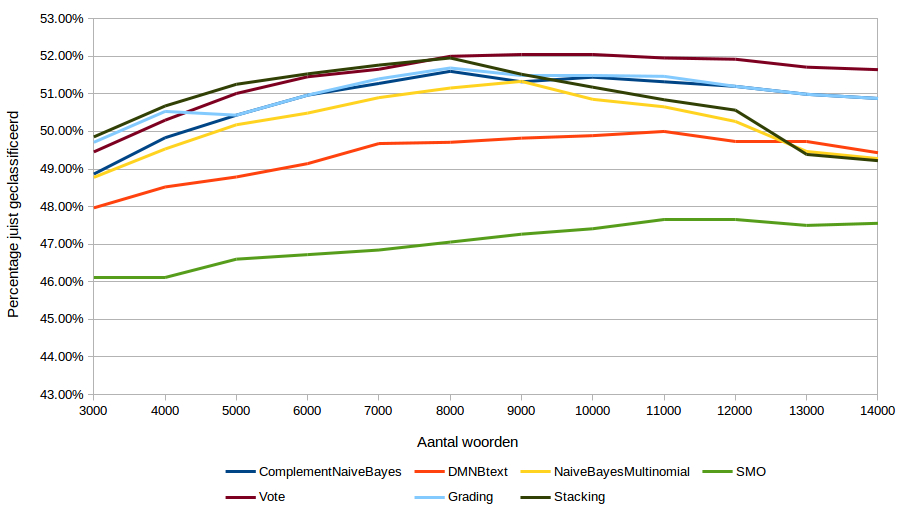
\includegraphics[width=\textwidth]{fig/classificatie-20000-wiki.jpg}
\end{figure}

De meest optimale classifier die voor dit probleem werd gevonden is het vote-algoritme (52,04\%) met de top 4 classifiers: ComplementNaiveBayes, DMNBtext, NaiveBayesMultinomial en SMO.


\subsection{Classificatie in subcategorie\"en (dataset Wikipedia)}
Voor elke subcategorie van de Wikipedia dataset werd ook de beste classifier gezocht. De resultaten zijn te vinden in tabel \ref{tab:wiki-sub}. Ook in deze classificatie is de gebruikte classifier erg afhankelijk van het classificatieprobleem. Er kan hier wel opgemerkt worden dat veel meer subklasses gevonden kunnen worden onder de meeste hoofdcategorie\"en dan in de vorige dataset het geval was. Dit draagt uiteraard bij aan de moeilijkheid van de classificat

\begin{table}[htbp] 
\centering 
\caption{Best scorende classifiers voor elke subcategorie van dataset Wikipedia} 
\begin{tabular}{rrrrr} \toprule & subklasses & woorden & classifier & correct \\ \midrule cultuur & 40 & 8000 & Vote & 45.83\% \\ geschiedenis & 21 & 3000 & NaiveBayesMultinomial & 37.65\% \\ heelal & 4 & 1000 & ComplementNaiveBayes & 78.75\% \\ mens en maatschappij & 40 & 9000 & Vote & 44.39\% \\ natuur & 14 & 1000 & Vote & 49.19\% \\ religie & 23 & 1000 & NaiveBayesMultinomial & 53.40\% \\ techniek & 28 & 5000 & ComplementNaiveBayes & 58.66\% \\ wetenschap & 28 & 4000 & StackingC & 55.99\% \\ \bottomrule 
\end{tabular}% 
\label{tab:wiki-sub}% 
\end{table}%

\section{Clustering}
Clustering is een methode die gebruikt wordt om documenten met gelijkaardige inhoud in eenzelfde cluster te groeperen \cite{Hotho2005}. Het wordt naast classificatie toegepast om gelijkaardige documenten te vinden over de grenzen van de classificatie heen (documenten die aan verschillende categorie\"en toebehoren, maar bv. over dezelfde persoon handelen). Ook zal clustering ervoor zorgen dat documenten binnen dezelfde categorie toch nog verder opgedeeld kunnen worden in bepaalde topics. Op deze manier kan meer informatie uit de teksten gehaald worden en die informatie kan op zijn beurt gebruikt worden door het aanbevelingssysteem. 

Elke cluster bevat een aantal documenten. Het is belangrijk dat documenten in een bepaalde cluster gelijkaardig zijn aan elkaar, maar verschillen met documenten in andere clusters. Cluster methodes groeperen documenten op basis van hun distributie in een bepaalde documentenruimte. We krijgen zo bijvoorbeeld een $n$-dimensionele ruimte als we het vector space model zouden gebruiken.

Clustering wordt berekend op basis van attributen van de tekst. Nochtans is het concept \quotes{cluster} een subjectief begrip. Wat de ene persoon ziet als een goede en relevante cluster, kan door iemand anders niet als een goede cluster aanzien worden. Clustering vraagt bijgevolg om een duidelijk evaluatiecriterium (zie \ref{evaluatie-clustering}), zodat we objectief kunnen vaststellen wat een goede cluster is.

\subsection{k-means clustering algoritme}
Een populair clustering algoritme is het k-means clustering algoritme (ook wel het algoritme van Lloyd genoemd \cite{Lloyd1982}). Voor een gegeven dataset $X = {x_1,...x_n}, x_n \in R^d$ wordt geprobeerd om deze data in $M$ verschillende subsets (clusters) $C_1,...,C_M$ te partitioneren, zodat een bepaalde clustervoorwaarde voldaan is \cite{Likas2011}. Het algoritme verwacht daarvoor een bepaalde waarde voor het aantal clusters $k$ die moeten gevormd worden. Deze $k$ zorgt voor heel wat belemmeringen bij het uitvoeren van dit algoritme, vooral omdat het vooraf niet duidelijk is hoe groot clusters zullen of kunnen worden en omdat dit voor elke documentencollectie anders ligt. Als een $k$ te klein wordt genomen zullen artikels die ver van elkaar liggen toch samen geclusterd worden. Als we de $k$ te groot nemen zullen de onderwerpen misschien onnodig opgesplitst worden in (te) kleine clusters.

Daarom wordt in eerste instantie het k-means algoritme iteratief uitgevoerd voor elke waarde van $k$. Het nadeel van elke $k$ iteratief uit te proberen is uiteraard de uitvoeringstijd bij grote documentencollecties. Om deze te beperken worden een aantal verschillende methodes uitgeprobeerd met als doel de uitvoeringstijd te verlagen (zie \ref{spark}, \ref{mahout}). 

Een tweede probleem bij het k-means clustering algoritme is dat het steeds opnieuw op zoek moet gaan naar de optimale clustercentra. Daartoe moeten een aantal iteraties ingesteld worden waarin het algoritme vervolgens op zoek gaat naar de ideale centra. De clusters worden in eerste instantie random gekozen en proberen vervolgens de inter-clusterafstand (tussen verschillende clusters) te vergroten en de intra-clusterafstand (tussen punten binnen dezelfde cluster) te verkleinen. Omdat dit een proces is dat veel tijd in beslag neemt wordt in \ref{mahout} een oplossing voorgesteld die dit probeert te minimaliseren. 

\subsection{Evaluatiecriteria voor clustering}\label{evaluatie-clustering}
Er bestaan twee manieren om resultaten van clustering te evalueren. Enerzijds kunnen statistische functies gebruikt worden om de eigenschappen van de clustering te beschrijven. Anderzijds kan classificatie gebruikt worden als \quotes{golden standard}, waarbij de clustering vergeleken wordt met de gegeven classificatie. Omdat het doel van de clustering in deze toepassing echter niet is om classificatie door te voeren, zijn we aangewezen op de statistische functies. Om te bepalen wat een goede cluster is, moeten we voor het k-means algoritme bepalen hoeveel clusters $k$ een dataset bevat. Hiervoor worden enkele criteria besproken.

\subsubsection{Vuistregel}
De vuistregel \cite{Science2013} is een simpele regel, die toegepast kan worden op elke gegeven dataset. De uitkomst van deze regel wordt enkel als een indicatie beschouwd en kan zeker niet gebruikt worden voor het bepalen van het effectieve aantal clusters. 
\begin{equation}
k = \sqrt{\frac{n}{2}}
\end{equation}

\subsubsection{Elbow method}
De \quotes{elbow method} \cite{Science2013} is een visuele methode. Het idee is om alle waarden van $k$ te itereren en telkens een kostenfunctie te plotten op een grafiek. Bij een bepaalde waarde van $k$ daalt de kost sterk, waarna het een plateau bereikt als $k$ verder ge\"itereerd wordt. 

Het is echter niet altijd gemakkelijk om deze \quotes{elbow} te vinden, zeker niet indien de documentencollectie groot wordt. Ze vereist enerzijds dat we alle clusters aflopen, maar vereist anderzijds ook dat een functie kan gemaakt worden die de optimale $k$ kan vinden. Die functie werd gevonden in \cite{Tibshirani2001} met de zogenaamde \quotes{Gap statistic}. Deze methode is echter niet bruikbaar voor grote documentencollecties omdat ze vereist dat eerst alle clusters worden gevonden, voor de optimale $k$ kan bepaald worden. 

\subsubsection{Inter- versus intra-cluster afstand}
Dit criterium werd voorgesteld in o.a. \cite{Ray} en probeert om de som van de kwadratische afstanden van alle punten tot hun clustercentrum te minimaliseren. Hiervoor moeten we de afstanden van elk document tot clustercentrum berekenen. Deze worden gegeven door:

\begin{equation}
intra = \frac{1}{N}\sum_{i=1}^{K}\sum_{x\in{C_i}}^{} \vert\vert \mathbf{x-z_i} \vert\vert ^2 
\end{equation}
waarbij $N$ het aantal documenten is in de documentencollectie, $K$ het aantal clusters en $z_i$ het cluster centrum van cluster $C_i$.

Vervolgens berekenen we de inter-cluster afstand. We berekenen dit als het minimum van de afstanden tussen de cluster centra:

\begin{equation}
intra = min(\vert\vert \mathbf{z_i-z_j}\vert\vert^2) ; i = 1,2,...,K-1 ; j = i+1, ..., K
\end{equation}

Van deze reeks hebben we enkel het minimum nodig, omdat we deze waarde willen maximaliseren. De andere clusters liggen sowieso verder van elkaar.

We combineren beide waarden vervolgens tot de \quotes{validity measure}:

\begin{equation}
validity = \frac{intra}{inter}
\end{equation}

Omdat de intra-cluster afstand steeds geminimaliseerd moet worden en de inter-cluster afstand steeds gemaximaliseerd, moet de validity measure telkens geminimaliseerd worden (minimum van de teller delen door maximum in de noemer zorgt voor minimalisatie van de validity measure). Omdat deze validity measure steeds daalt wordt een bepaalde \textit{treshold} ingesteld, zodat de clusters niet te specifiek worden (en dus heel weinig relevante buren zouden overhouden). Deze waarde wordt experimenteel bepaald in tabel \ref{tab:clusters-validity} voor een kleine dataset (20 documenten). Daarbij wordt het iteratieve k-means clustering algoritme toegepast op de dataset en bij elke uitvoer de validity-measure nagekeken. De teksten zijn gekozen uit de dataset van Het Laatste Nieuws en zijn zo geselecteerd dat er artikels van 5 totaal verschillende topics aanwezig zijn (de zwangerschap van Angelina Jolie, Osama Bin Laden, transfers van voetbalploeg Anderlecht, Maddie McCan en de Amerikaanse presidentsverkiezingen).

Het clusteralgoritme dat gebruikt wordt past k-means clustering toe met een feature vector van 1000 features. Het algoritme krijgt 100 iteraties om de optimale clustercentra te bepalen voor k-means en dit voor elke $k$. Iedere iteratie wordt a.d.h.v. de vooraf opgestelde lijst van topics vergeleken met hoe de clustering presteert. Naast de euclidische afstand wordt nog een andere afstandsfunctie \cite{Huang2008} gebruikt: cosine similary. Deze zou beter presteren voor tekstuele data. Bij de cosine similary \cite{Owen2011} worden punten voorgesteld als vectoren van de oorsprong naar het punt in de ruimte. Twee vectoren vormen op die manier een bepaalde hoek $\theta$. Wanneer die hoek klein is liggen de punten enigszins dicht bij elkaar. De cosinus van die hoek ligt dicht bij 1 wanneer de hoek klein is en wordt kleiner wanneer de hoek groter wordt. De cosine similary functie trekt de waarde van de cosinus af van 1 om een afstand te bekomen. Deze is dus 0 indien de punten dicht van elkaar liggen en wordt groter naar mate de punten verder uit elkaar liggen. De formule voor twee n-dimensionele vectoren $(a_1, a_2, ... , a_n)$ en $(b_1, b_2, ... , b_n)$ is:

\begin{equation}
d = 1 - \frac{(a_1b_1+a_2b_2+ ... + a_nb_n)}{\sqrt{a_1^2 + a_2^2 + ... + a_n^2} \sqrt{b_1^2 + b_2^2 + ... + b_n^2}}
\end{equation}

\begin{table}[htbp]
  \centering
  \caption{Berekenen van de validity-measure voor verschillende afstandsfuncties (euclidische afstand, cosine similary) bij k-means algoritme (1000 features, 100 iterations)}
    \begin{tabular}{rrrr}
    \toprule
    \multicolumn{1}{c}{k} & euclidische afstand & cosine similarity \\
    \midrule
    1     & 1.80  & 1.80  \\
    2     & 0.48   & 1.13 \\
    3     & 0.20  & 0.63  \\
    4     & 0.17   & 0.61   \\
    5     & 0.17  & 0.51  \\
    6     & 0.17  & 0.42   \\
    7     & \textbf{0.16}  & 0.37  \\
    8     & 0.12  & \textbf{0.33}  \\
    9     & 0.12  & 0.29  \\
    10    & 0.12  & 0.21   \\
    11    & 0.10  & 0.22  \\
    12    & 0.09  & 0.19   \\
    13    & 0.07  & 0.15   \\
    14    & 0.05  & 0.13    \\
    15    & 0.04  & 0.09   \\
    \bottomrule
    \end{tabular}%
  \label{tab:clusters-validity}%
\end{table}%

De subjectief bepaalde optimale validity measures zijn in het vet aangeduid. Dit zijn de validity measures waarbij de topics het best lijken op de vooropgestelde topics (of delen daarvan). Zoals verwacht komt de cosine similary het dichtst in de buurt van de effectieve topics. Geen enkel algoritme slaagt er echter in de vooropgestelde 5 topics te detecteren. Omdat de cosine similary het best presteert wordt verder gewerkt met deze afstandsfunctie.

\subsection{Named entity recognition}
Veel van de clusters die geconstrueerd worden handelen over een bepaald onderwerp. In de recente actualiteit zouden we bijvoorbeeld een cluster rond ISIS kunnen vinden die handelt over terrorisme. Die bepaalde cluster zou ge\"identificeerd kunnen worden door zogenaamde \textit{named entities} van personen binnen deze organisatie, personen die aanslagen pleegden, de plaatsen waar aanslagen plaatsvonden, etc.

Dit idee werd ge\"introduceerd door o.a. \cite{Montalvo2015}, waar een systeem gebouwd werd dat artikels clusterde uit twee verschillende talen door gebruik te maken van \textit{natural language processing} (NLP) en named entity recognition. Zij gaan uit van het idee dat een artikel (en bij uitbreiding een tekst) geschreven is met zes vragen in het achterhoofd: wat, wie, wanneer, waar, waarom en hoe. Een belangrijk deel van deze vragen kan beantwoord worden met een named entity (NE). Antwoorden op \textit{waar} geven bijvoorbeeld namen van locaties, terwijl wanneer een datum of tijd teruggeeft. Als ervan uit gegaan wordt dat:
\begin{itemize}
\item NE's over verschillende, gelijkaardige documenten behouden blijven omdat het moeilijk is om een naam te parafraseren,
\item de frequentie van NE's in zinnen de belangrijkheid benadrukt van gebeurtenissen waar ze mee geassocieerd zijn,
\item twee verschillende verhalen met dezelfde NE's meer dan waarschijnlijk aan dezelfde topic toebehoren,
\end{itemize} dan kan een model gemaakt worden dat specifieke clusters rond deze NE's kan bouwen.

Omdat het gemakkelijker ligt om topics te vinden rond personen (PERS), organisaties (ORG), locaties (LOC) en andere (MISC) worden enkel deze NE's gebruikt voor het model. Andere categorie\"en zoals tijd, datum of cijfers worden niet als belangrijk gezien omdat ze een hoge kans geven op extra ruis als ze niet voorzichtig gebruikt worden. Er kunnen bijvoorbeeld twee belangrijke gebeurtenissen in de geschiedenis gebeurd zijn op hetzelfde tijdstip, maar de gebeurtenissen kunnen totaal verschillen. Zeker bij datasets zoals die van Het Laatste Nieuws, waar veel topics op dezelfde dag worden behandeld, moet daarvoor opgelet worden. 

Sommige auteurs veronderstellen echter dat documenten clusteren enkel rond NE's schadelijk kan zijn voor clustering (o.a. \cite{Friburger2002}, \cite{Gliozzo2005}). Ze veronderstellen dat NE's alleen niet genoeg informatie geven over een tekst om een dataset correct te clusteren. Een voorbeeld hiervan is een tekst over tuinieren, waarin aangegeven wordt dat hagen moeten gesnoeid worden rond deze periode van het jaar, welke planten gezaaid kunnen worden, etc. Deze tekst bevat geen NE's en kan dus niet geclusterd worden. Daarom wordt in dit geval een model gebruikt waarin NE's een belangrijkere rol krijgen dan andere features. Nadat de documentencollectie het stadium van preprocessing doorlopen heeft en de feature vector wordt opgebouwd, krijgen NE's een groter gewicht toegekend dan de andere features. 

\subsubsection{Implementatie van NLP}
Om NE's uit een tekst te halen wordt gebruik gemaakt van de Stanford Named Entity Recognizer \cite{Finkel2005} met een Nederlandse classifier. Binnen dit systeem worden NE's getagd als volgt: PER (personen), ORG (organisaties), LOC (locaties) en MISC (andere). Door de term frequency van deze NE's te verhogen worden ze belangrijker voor een tekst en wordt geprobeerd om een betere clustering te verkrijgen. 

Omdat deze classifier enkel voor het Nederlands werkt, zijn er voor deze classifier geen grote evaluatiesets beschikbaar. Daarom wordt een set van 1930 woorden zelf getagd waarop vervolgens ge\"evalueerd wordt. De globale precisie van deze classifier was 97,31\% (1878/1930 objecten werden correct getagd). De individuele scores kunnen gevonden worden in tabel \ref{tab:nlp-classifier}. 

\begin{table}[htbp]
  \caption{Precisie van een Nederlandse classifier voor Stanford NLP}
  \centering
    \begin{tabular}{rrrrrr}
    \toprule
          & Aantal tags & antwoorden & Precisie & Recall & F-score \\
    \midrule
    LOC   & 26    & 22    & 0.95  & 0.81  & 0.88 \\
    PER   & 30    & 28    & 0.75  & 0.7   & 0.72 \\
    MISC  & 22    & 18    & 0.67  & 0.55  & 0.6 \\
    ORG   & 7     & 17    & 0.35  & 0.85  & 0.5 \\
    O     & 1845  & 1793  & 0.97  &       &  \\
    \bottomrule
    \end{tabular}%
  \label{tab:nlp-classifier}%
\end{table}%

De NLP wordt ge\"integreerd tijdens de preprocessing. Tussen de stap van tokenization en stopwoordfiltering komt een extra stap die de NE's uit een tekst een hogere frequentie geeft tegenover de andere elementen. Op die manier wordt een woord belangrijker voor een tekst en wordt verwacht dat hij vaker als discriminerende factor zal dienen bij het clusteren. 

\subsubsection{Resultaten voor kleine datasets}
Er wordt terug gegrepen naar de dataset met 20 documenten en 5 topics uit de vorige sectie. Opnieuw wordt dezelfde clustering toegepast, maar krijgen de named entities deze keer een groter gewicht. De volgende clustering kan gevonden worden met een validity measure van 0.31:
\\

\begin{lstlisting}
Cluster 0
  Document: 0, Title: Pakistan niet op zoek naar bin Laden
  Document: 5, Title: Hoe Osama bin Laden de Amerikanen ontglipte in 2001
  Document: 8, Title: Zoon Bin Laden wil in Groot Brittannie wonen
  Document: 13, Title: Bin Laden junior wil dat pa ermee kapt
Cluster 1
  Document: 1, Title: Anderlecht verhuurt Cyril Thereau aan Charleroi
  Document: 12, Title: Anderlecht huurt Yakovenko
  Document: 16, Title: Anderlecht strikt Guillaume Gillet
  Document: 18, Title: Luigi Pieroni naar Anderlecht
Cluster 2
  Document: 2, Title: McCanns onderhandelen over verfilming Maddie
  Document: 3, Title: McCanns verdenken politie onderzoek te vertragen
  Document: 14, Title: McCanns verspreiden foto van mogelijke ontvoerder
  Document: 19, Title: Foto van kidnapper is afleidingstruc van McCanns
Cluster 3
  Document: 4, Title: Angelina is zwanger geen twijfel mogelijk
  Document: 6, Title: Angelina zwanger van tweeling
  Document: 10, Title: Jurk Angelina wakkert geruchten over zwangerschap aan
  Document: 11, Title: Angelina Jolie en Brad Pitt oefenen voor tweede kind
Cluster 4
  Document: 7, Title: Analyse waarom South Carolina Obama zuur kan opbreken
  Document: 9, Title: Clinton en Obama strijden in South Carolina
  Document: 15, Title: Clinton en McCain op kop in race naar Witte Huis
  Document: 17, Title: Analyse Wie is John McCain
\end{lstlisting}

Door het gebruik van NE's wordt de vooropgestelde clustering perfect gevonden in de kleine dataset. Deze clustering wordt vervolgens getest op een grotere dataset in de volgende paragraaf.

\subsubsection{Resultaten voor grote datasets}
Het clusteralgoritme met NLP wordt toegepast op een dataset met 10121 documenten (Het Laatste Nieuws, januari 2008). De validity measure wordt op 0,32 gezet en het algoritme wordt uitgevoerd met iteratieve $k$ (1000 features, 100 iteraties om cluster centra te bepalen). Van bij het begin kunnen we opmerken dat dit algoritme niet zal kunnen gebruikt worden voor grote hoeveelheden data. De totale tijd die nodig is om clusters te maken stijgt bijna exponentieel en neemt al snel een uur in beslag om 25 clusters te vinden (zie afbeelding \ref{fig:clustering-10000-exp}). Op dat moment krijgt de clustering een validity measure van 0,93 en zijn de clusters dus nog niet gevormd.

\begin{figure}[h]
	\caption{Aantal clusters in het iteratieve k-means algoritme in relatie tot het aantal clusters voor een dataset met 10121 documenten}
	\label{fig:clustering-10000-exp}	
	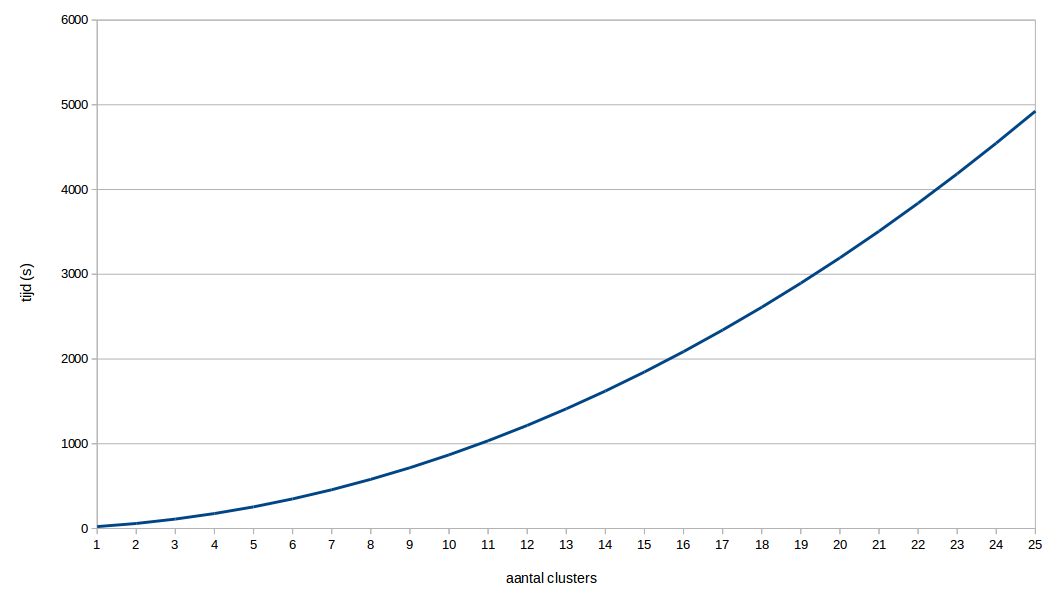
\includegraphics[width=\textwidth]{fig/clustering-10000-exp.png}
\end{figure}

Om de totale tijd die het algoritme nodig heeft te doen dalen worden twee implementaties voorgesteld. De eerste in Apache Spark (zie \ref{spark}) en een tweede in Apache Mahout (zie \ref{mahout}). Beiden werken bovenop het Hadoop filesysteem om sneller te kunnen werken en mogelijk gemakkelijker te schalen bij groter wordende datacollecties. Bovendien ondersteunen beide systemen enkele vormen van clustering. 

\subsection{Implementatie van k-means met Apache Spark}\label{spark}
Apache Hadoop \cite{hadoop} is een open-source framework dat oplossingen biedt voor big data, samen met uitgebreide verwerkings- en analysetools. Hadoop bestaat uit twee grote componenten: HDFS (Hadoop Distributed File System) en MapReduce \cite{Dean}. HDFS is een schaalbaar, effici\"ent en replica-based opslagmedium voor data. Het is gebaseerd op een master-slave architectuur waar \quotes{namenode} de master is en de \quotes{datanodes} de slaves. De slaves bevatten ook de effectieve data. 

MapReduce zorgt ervoor dat gerepliceerde data snel en parallel verwerkt kan worden volgens map en reduce fases. \textit{Map} is de fase die gebruikt wordt om in parallel de delen van het gedistribueerd systeem op te halen via verschillende \textit{mappers}. De outputs van de mappers wordt door sorteer- en shufflealgoritmes gehaald om in de \textit{reduce} fase de data te aggregeren en het resultaat te vinden van het initieel probleem.

Apache Spark werd ontwikkeld in het UC Berkeley AMPLab en werd open-source in 2010. Het is ontworpen voor effici\"ente gegevensverwerking en bied een gebruiksvriendelijke interface aan om zo tot betere oplossingen te komen voor big data toepassingen. Spark heeft sinds 2012 bovendien een set robuuste en schaalbare leeralgoritmes onder de naam \quotes{MLlib} aan boord en ondersteunt een veel breder gamma aan applicaties dan MapReduce, maar behoud daarbij wel zijn automatische fouttolerantie.
 
Spark werkt met RDDs (Resilient distributed Datsets) om efficiente applicaties te ondersteunen. RDDs kunnen opgeslagen worden in het geheugen tussen query's zonder dat replicatie nodig is. Indien data verloren gaat wordt deze opnieuw opgebouwd gebruik makend van \textit{lineage}: elke RDD herinnert hoe het gebouwd is van een andere dataset en kan zichzelf zo herbouwen. Op die manier presteert Spark beter dan alle bestaande modellen.

Apache Spark biedt in zijn MlLib een k-means algoritme aan. Dit werd getest in \cite{Gopalani2015a} en werkt tot drie keer sneller dan hetzelfde algoritme gebruik makend van MapReduce. De implemenatie is hier wel zo dat er geen gebruik kan gemaakt worden van een alternatieve afstandsfunctie. Om voor de snelheid van Apache Spark te kiezen zijn we dus verplicht over te stappen naar de Euclidische afstandsfunctie.

Een vergelijking in tijd om de eerste 25 clusters te maken bij de k-means implementatie van Apache Spark (met 1000 features en 100 iteraties) en het eenvoudige algoritme dat hiervoor reeds gebruikt werd kan gevonden worden in figuur \ref{fig:sparkvskmeans}. 

\begin{figure}[h]
	\caption{Vergelijking tussen de tijd om k-means clustering door te voeren in Apache Spark en binnen een eenvoudig algoritme}
	\label{fig:sparkvskmeans}	
	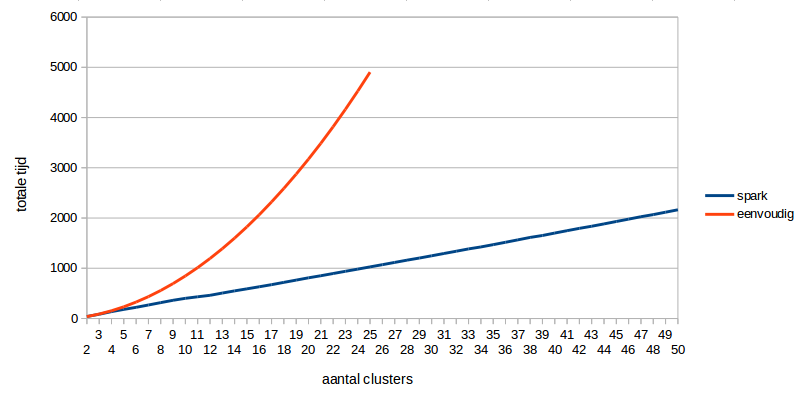
\includegraphics[width=\textwidth]{fig/sparkvsclustering.png}
\end{figure}

De grafiek van het eenvoudige algoritme is dezelfde als in figuur \ref{fig:clustering-10000-exp}, maar we merken vooral de quasi lineaire tijd van Apache Spark op. Deze doet er gemiddeld 44 seconden over om een clustering uit te voeren in de eerste 50 clusters, terwijl het eenvoudige algoritme al 377 seconden nodig had om cluster 25 te vormen. Door Apache Spark te gebruiken kan de rekentijd dus flink beperkt worden, maar ten koste van het gebruik van de cosine similary. Om de effici\"entie van dit algoritme te combineren met de positieve invloed van de cosine similary wordt een nieuwe implementatie in Apache Mahout voorgesteld in de volgende sectie.

\subsection{Implementatie van k-means met Apache Mahout}\label{mahout}
Apache Mahout \cite{Owen2011} is een open-source machine learning library van Apache. Het ondersteunt recommender engines met collaborative filtering, clustering en classificatie. Ook is het erg schaalbaar en werkt (zoals Apache Spark) bovenop Apache Hadoop. Bovendien wordt Mahout als Java library aangeboden, waardoor deze eenvoudig in de workflow kan worden opgenomen.

Mahout biedt een methode om k-means clustering te verbeteren aan de hand van \textit{Canopy Centers}. Hiervoor werd de optimale $k$ steeds bepaald door alle waarden voor $k$ iteratief af te lopen en op basis daarvan de optimale waarde te selecteren. Alhoewel deze methode met enige zekerheid een optimale $k$ zal vinden, is dit zeker niet snel en bijgevolg moeilijk bruikbaar voor zeer grote datasets. Dat probleem wordt natuurlijk evenredig groter met een groter wordende dataset. 

De implementatie van het Canopy algoritme kan gevonden worden in \cite{McCallum2000}. Het basis-idee is dat het aantal berekeningen die nodig zijn om afstanden te berekenen sterk kan verminderen door de data eerst te verdelen in overlappende subsets en daarop de afstanden te berekenen tussen paren van items die aan dezelfde subset toebehoren. De sterkte van het algoritme ligt vooral in de snelheid waarmee clusters gevormd worden. Die sterkte is ook meteen de grootste zwakte van het algoritme, want de clusters die gevormd worden bij het Canopy algoritme zijn niet altijd zeer accuraat. Toch kan op deze manier het optimale aantal clusters $k$ bepaald worden. Die $k$ clusters dienen vervolgens als input voor het k-means algoritme dat wel in staat is om de goede clusters te vinden.

Het Canopy algoritme moet eerst notie krijgen van hoe groot de clusters zijn waar naar op zoek gegaan wordt. Daarvoor worden twee variabelen ge\"introduceerd: $T_1$ en $T_2$. Dit zijn twee tresholds voor afstand met $T_1 > T_2$. Het algoritme begint met een dataset van punten en lege lijst \textit{canopies}. Er wordt ge\"itereerd over de dataset en bij elke iteratie wordt een punt van de dataset verwijderd en wordt een canopy aan de lijst toegevoegd met dat punt als centrum. Vervolgens worden de rest van de punten een voor een afgelopen en wordt telkens de afstand van dat punt tot alle canopy centra berekend. Als die afstand binnen $T_1$ valt, wordt dit punt toegevoegd aan de canopy. Als de afstand bovendien binnen $T_2$ valt wordt het verwijderd van de lijst. Dit om te voorkomen dat een nieuwe canopy zou aangemaakt worden in de opeenvolgende loops. Dit proces loopt tot de lijst leeg is. 

Om te bepalen wat een goede waarde is voor $T_1$ en $T_2$ wordt nog even teruggegrepen naar de dataset met 20 artikels. In die dataset moeten 5 clusters gevormd worden. Om dat te bereiken wordt $T1$ gevarieerd van 0 tot 1 met iteraties van 0,01 (de cosine similary geeft immers enkel waarden aan tussen 0 en 1). Telkens wordt daarbij ook de bijhorende $T_2$ ge\"itereerd ($T_2 \leq T_1$ en per 0,01). De output van dit algoritme wordt vervolgens als input voor k-means gebruikt en levert een bepaalde validity measure op. De belangrijkste resultaten zijn te vinden in tabel \ref{tab:canopy}. In die tabel worden alle waarden voor $T_1$ en $T_2$ opgesomd die de gezochte clustering opleveren voor deze kleine dataset.

\begin{table}[htbp] 
\centering 
\caption{Iteratie van de treshold parameters voor Canopy clustering ($T_1$ en $T_2$) die voor een documentenset van 20 documenten de 5 topics al dan niet correct detecteren met het k-means algoritme} 
\begin{tabular}{rrrrr} 
 \toprule $T_1$ & $T_2$ & clusters & validity & correct \\ \midrule 0.96 & 0.92 & 5 & 0.64 & ja \\ 0.96 & 0.93 & 5 & 0.64 & ja \\ 0.96 & 0.94 & 5 & 0.67 & nee \\ 0.96 & 0.95 & 5 & 0.67 & nee \\ 0.97 & 0.92 & 5 & 0.64 & ja \\ 0.97 & 0.93 & 5 & 0.64 & ja \\ 0.97 & 0.94 & 5 & 0.68 & ja \\ 0.97 & 0.95 & 5 & 0.68 & ja \\ 0.97 & 0.96 & 5 & 0.68 & ja \\ 0.98 & 0.92 & 5 & 0.68 & ja \\ 0.98 & 0.93 & 5 & 0.68 & ja \\ 0.98 & 0.94 & 5 & 0.71 & nee \\ 0.98 & 0.95 & 5 & 0.71 & nee \\ 0.98 & 0.96 & 5 & 0.71 & nee \\ 0.98 & 0.97 & 5 & 0.71 & nee \\ 0.99 & 0.92 & 5 & 0.70 & nee (*) \\ 0.99 & 0.93 & 5 & 0.70 & nee (*) \\ 0.99 & 0.94 & 5 & 0.70 & nee \\ 0.99 & 0.95 & 5 & 0.70 & nee \\ 0.99 & 0.96 & 5 & 0.70 & nee \\ 0.99 & 0.97 & 5 & 0.70 & nee \\ 1 & 0.92 & 5 & 0.68 & nee \\ 1 & 0.93 & 5 & 0.68 & nee \\ \bottomrule
\end{tabular}% 
\label{tab:canopy}% 
\end{table}%

Niet alle opgesomde waarden voor $T_1$ en $T_2$ leveren de optimale (correcte) clustering op. De waarden met een (*) geven wel een aanvaardbare clustering, maar splitsen de topic rond het presidentschap in Amerika nog verder op in Obama en Clinton enerzijds en McCain anderzijds. Omdat deze clustering heel specifiek is, terwijl die twee clusters toch heel nauw verwant zijn krijgen we daar een minder goede validity measure. Ook is het wenselijk dat de cluster deze artikels samen zou nemen, aangezien een gebruiker die ge\"interesseerd is in een artikel rond Obama hoogstwaarschijnlijk ook zal ge\"interesseerd zijn in de andere presidentskandidaten. 

Mahout laat ook toe om de belangrijkste termen per cluster op te sommen. Dit gegeven kan mogelijk ook interessant zijn voor de recommender. Door deze belangrijke termen te verzamelen kan wat een gebruiker belangrijk vindt ook toegevoegd worden aan de vergelijking die uitzoekt welke artikels een gebruiker mogelijk interessant kan vinden. Enkele belangrijke termen voor het topic rond de Amerikaanse presidentsverkiezingen zijn bijvoorbeeld de volgende: carolina, obama, zwart, mccain, senator, clinton, peiling. Dit is een goede combinatie van sterke keywords en named entities die ons in staat kunnen stellen om andere artikels gemakkelijk aan te bevelen. 

Vervolgens wordt deze methode toegepast op de dataset van Het Laatste Nieuws uit Januari 2008 (10121 documenten). De waardes voor de canopy worden gekozen gelijkaardig aan die uit tabel \ref{tab:canopy} ($T_1=0,96$ en $T_2=0,92$). De uitvoeringstijd van dit algoritme blijft onder de 15 minuten (inclusief preprocessing voor 10121 documenten). Deze clustering levert 1685 clusters op, met dus een gemiddelde inhoud van ongeveer 6 artikels per cluster. 

\subsection{Fuzzy k-means clustering}
Fuzzy k-means laat toe om aan \textit{overlapping} clustering te doen in plaats van \textit{exclusive} clustering. Terwijl k-means de harde clusters zoekt (waar elk punt aan \'e\'en cluster toebehoort), kan fuzzy k-means soft clusters ontdekken. Items behoren daarbij aan meerdere clusters toe met een bepaalde zekerheid. Deze zekerheid is een uitdrukking van de afstand die een punt heeft tot het centrum van een cluster. 

Fuzzy k-means is een algoritme dat beschikbaar is in Apache Mahout. Dit algoritme neemt een belangrijke parameter: de \textit{fuzziness factor} $m$ (groter dan 1). Stel dat voor een vector $V$ de afstanden tot elke van de $k$ clusters gegeven zijn door $d_1,d_2,...,d_k$. De fuzziness factor wordt dan gebruikt bij het bepalen van de graad van verbinding $u_1$ van een vector $V$ tot de eerste cluster $C_1$:

\begin{equation}
u_i = \frac{1}{\frac{d_1}{d_1}^{\frac{2}{m-1}}+\frac{d_1}{d_2}^{\frac{2}{m-1}}+...+\frac{d_1}{d_k}^{\frac{2}{m-1}}}
\end{equation} 

De graad van verbinding tot een andere cluster kan gevonden worden door $d_1$ in de tellers van de uitdrukking in de noemer te vervangen door een andere cluster. 

Enerzijds zullen bij een waarde 2 voor $m$ alle graden van verbinding 1 worden. Anderzijds, als $m$ dichter bij 1 komt zal meer belangrijkheid gegeven worden aan de cluster die het dichtst bij de vector ligt. Fuzzy k-means gedraagt zich bijgevolg meer als k-means wanneer de waarde voor $m$ dicht bij 1 komt te liggen. Als $m$ groter wordt zal de fuzziness van het algoritme verhogen en zal meer overlap merkbaar zijn. 

Voor het bepalen van het aantal clusters wordt dezelfde methode gevolgd als bij k-means clustering ($k$ zoeken via Canopy algoritme, clustering uitvoeren met Fuzzy k-means met dezelfde clustercentra). Fuzzy k-means steunt immers op hetzelfde principe als normale k-means. 

Het voordeel om Fuzzy k-means te gebruiken tegenover de normale k-means is dat een bepaald item beter gesitueerd kan worden. Een item dat gaat over ISIS, terrorisme en aanslagen kan zowel bij een cluster geplaatst worden rond de aanslagen in Brussel als bij een cluster rond de aanslagen in Parijs. Bij normale k-means zouden deze artikels misschien samen geclusterd worden, omdat de inhoud min of meer overeen komt. Met Fuzzy k-means kan de specificiteit van een cluster verhoogd worden om zo toch een onderscheid te maken tussen beide gebeurtenissen. Op die manier kan met kleinere topics dus soms meer informatie gehaald worden uit dezelfde data. Dit is dus zeker interessant in het kader van aanbevelingen. De gebruiker kan zo tussen verschillende aaneensluitende topics \quotes{springen} die hem waarschijnlijk ook zullen interesseren. 

Als we Fuzzy k-means toepassen op de kleine dataset van 20 documenten krijgen we eveneens 6 clusters (gebruik makend van dezelfde waarden voor canopy clustering uit de vorige sectie). De resultaten zijn echter minder kwalitatief dan bij normale k-means. Een artikel over Osama bin Laden wordt zo toch met een hoge waarschijnlijkheid geclusterd bij een artikel van de zwangerschap van Angelina Jolie. Als we dit bekijken in termen van een aanbevelingssysteem, dan kunnen we deze clustering niet toestaan. Het is de bedoeling dat gebruikers artikels krijgen aangeraden die zeer relevant zijn tegenover hun huidige voorkeuren. Bij fuzzy k-means is dit niet gegarandeerd. 

\subsection{Conclusie voor clustering}
Door de schaalbaarheid naar meerdere machines, uitbreidbaarheid van de algoritmes en algemene snelheid van Apache Mahout framework wordt sowieso voor deze implementatie gekozen. Het clusteralgoritme dat gebruikt wordt in dit systeem wendt het canopy algoritme aan en voedt daarmee het normale k-means algoritme met het optimale aantal clusters. De implementatie van het k-means algoritme maakt gebruik van de cosine similary om gerelateerde arikels te zoeken. Dit wordt gecombineerd met de opwaarding van named entities om in een goede clustering te voorzien.

\section{Aanbevelingssysteem}
Het gebruikte aanbevelingssysteem is een klassieke content-based recommender, gebouwd in Lenskit \cite{Ekstrand2011a}. In plaats van de manueel ingegeven tags wordt gebruik gemaakt van de verworven informatie uit zowel classificatie als clustering. Deze informatie wordt doorgegeven aan de recommender onder vorm van tags. Zo krijgt elk item een tag voor de hoofdcategorie, een tag voor de subcategorie en een of meerdere tags met de cluster of clusters waartoe het item behoort. Met deze data kan het content-based systeem gelijkaardige items vinden voor een bepaalde gebruiker. De resultaten en performantie van dit aanbevelingssysteem worden in hoofdstuk \ref{resultaten} besproken.